% =========================================================
% Template Laporan Kerja Praktik
% Departemen Teknik Elektro dan Teknologi Informasi
% Fakultas Teknik Universitas Gadjah Mada
% Disesuaikan untuk: Bagus Aldiguna dan Mirzariel Akmal Norman
% =========================================================
%!TEX program = xelatex
\documentclass[12pt,a4paper,onecolumn,oneside,final]{report}

%Isi identitas proyek akhir disini

\providecommand{\judulid}{Analisis Kelayakan Modul PV Pasca-Terendam di PLTS Terapung Cirata Menggunakan Pengujian Kurva I--V dan Indikator Arus--Tegangan}

\providecommand{\tempat}{PT Pembangkitan Jawa Bali Masdar Solar Energi (PT PMSE)} %Nama Perusahaan MBKM
\providecommand{\place}{company name} % Company Name MBKM

\providecommand{\penempatan}{Penempatan di perusahaan} %Penempatan lengkap di perusahaan

\providecommand{\penulis}{Bagus Aldiguna dan Mirzariel Akmal Norman}
\providecommand{\nim}{23/521708/TK/57563 dan 23/523162/TK/57824}
\providecommand{\penulisSatu}{Bagus Aldiguna}
\providecommand{\nimSatu}{23/521708/TK/57563}
\providecommand{\penulisDua}{Mirzariel Akmal Norman}
\providecommand{\nimDua}{23/523162/TK/57824}

\providecommand{\tglMulai}{5 Januari 2026}
\providecommand{\tglSelesai}{20 Februari 2026}
\providecommand{\penempatan}{PLTS Terapung Cirata, PT Pembangkitan Jawa Bali Masdar Solar Energi (PT PMSE)}

\providecommand{\tipe}{Laporan Kerja Praktik} %Tipe Laporan
\providecommand{\type}{Final Project} %Tipe Laporan
\providecommand{\prodi}{Program Studi Teknik Elektro} %Nama Prodi
\providecommand{\departemen}{Departemen Teknik Elektro dan Teknologi Informasi}
\providecommand{\fakultas}{Fakultas Teknik} %Nama Fakultas
\providecommand{\universitas}{Universitas Gadjah Mada} %Nama Universitas
\providecommand{\tglpengesahan}{\today} %Tanggal di Halaman Pengesahan
\providecommand{\tglpersetujuan}{\today} %Tanggal di Lembar Persetujuan
\providecommand{\tglpernyataan}{\today} %Tanggal di Surat Pernyataan

\providecommand{\tahun}{2026} %Tahun Proyek Akhir

\providecommand{\ketuapenguji}{Nama Ketua Penguji} %Nama Ketua Penguji
\providecommand{\NIPketuapenguji}{XXXXXXXXXXXXXXXXXX} %NIP Ketua Penguji

\providecommand{\sekretarispenguji}{Nama Sekretaris Penguji} %Nama Sekretaris Penguji
\providecommand{\NIPsekretarispenguji}{XXXXXXXXXXXXXXXXXX} %NIP Sekretaris Penguji

\providecommand{\anggotapenguji}{Nama Anggota Penguji} %Nama Anggota Penguji
\providecommand{\NIPanggotapenguji}{XXXXXXXXXXXXXXXXXX} %NIP Anggota Penguji

\providecommand{\dekan}{Nama Dekan.} %Nama Dekan
\providecommand{\NIPdekan}{XXXXXXXXXXXXXXXXXX} %NIP Dekan

\providecommand{\koordepartemen}{Prof. Ir. Hanung Adi Nugroho, S.T., M.E., Ph.D., IPM., SMIEEE.} %Nama Koordepartemen
\providecommand{\NIKAkoordepartemen}{XXXXXXXXXXXXXXXXXX} %NIKA Koordepartemen

\providecommand{\kaprodi}{Dr. Iswandi, S.T., M.Eng.} %Nama Koorprodi
\providecommand{\NIPkaprodi}{XXXXXXXXXXXXXXXXXX} %NIP Koorprodi

\providecommand{\pembimbing}{Dr.-Ing. Ir. Yohan Fajar Sidik, S.T., M.Eng.} %Nama Dosen Pembimbing
\providecommand{\NIPpembimbing}{111199001202205101} %NIP Dosen Pembimbing

\providecommand{\pimpinanPerusahaan}{Nama Lengkap dan gelar} %Nama Lengkap Pimpinan Perusahaan
\providecommand{\jabatanPimpinan}{Jabatan} %Jabatan Pimpinan Perusahaan

\providecommand{\pembimbingPerusahaan}{Ilman Rizky, M.T.} %Nama Pembimbing Magang
\providecommand{\jabatanPembimbing}{Plant Engineer} %Jabatan Pembimbing Magang

\providecommand{\katakunci}{kata kunci 1, kata kunci 2, kata kunci 2} %Kata kunci dalam Bahasa Indonesia
\providecommand{\keywords}{keyword 1, keyword 2, keyword 3} %Kata kunci dalam Bahasa Inggris

% =========================================================
% PREAMBLES.TEX - FINAL REPLACEMENT
% Untuk Laporan Kerja Praktik + Gambar Teknis PV
% Compile menggunakan XeLaTeX atau LuaLaTeX
% =========================================================

% --- PENGATURAN WARNA (HARUS DI ATAS) ---
% Memanggil xcolor di awal mencegah bentrok opsi dengan paket lain
\usepackage[table,xcdraw]{xcolor}

% --- PENGATURAN BAHASA DAN FONT ---
\usepackage[indonesian]{babel}

% Menggunakan font asli Times New Roman
% WAJIB compile dengan XeLaTeX atau LuaLaTeX, bukan pdfLaTeX
\usepackage{fontspec}
\setmainfont{Times New Roman}

% --- PENGATURAN SPASI DAN PARAGRAF ---
\usepackage{setspace}
\onehalfspacing

\usepackage{indentfirst}
\setlength{\parindent}{1cm}
\setlength{\parskip}{0pt}

\tolerance=1
\emergencystretch=\maxdimen
\hyphenpenalty=10000
\hbadness=10000

% --- PENGATURAN HALAMAN DAN MARGIN ---
\usepackage{geometry}
\geometry{
    top=3.5cm,
    left=3.75cm,
    bottom=2.5cm,
    right=2.75cm,
}

\usepackage{scrextend}
\usepackage{fancyhdr}
\usepackage{changepage}
\usepackage{pdflscape}
\usepackage{rotating}

% --- PENGATURAN LEVEL DAN PENOMORAN BAB/SUBBAB ---
\setcounter{secnumdepth}{6}

\renewcommand{\thesection}{\arabic{chapter}.\arabic{section}\hspace{0.05cm}}
\renewcommand{\thesubsection}{\arabic{chapter}.\arabic{section}.\arabic{subsection}\hspace{-0.25cm}}
\renewcommand{\thesubsubsection}{\Alph{subsubsection}.\hspace{-0.25cm}}
\renewcommand{\theparagraph}{\arabic{paragraph}.\hspace{-0.25cm}}

% --- PENGATURAN JUDUL BAB DAN SUBBAB ---
\usepackage{titlesec}

\titleformat{\chapter}
  {\doublespacing\fontsize{14pt}{16pt}\bfseries}
  {\MakeUppercase{\chaptertitlename\ \Roman{chapter}}\filcenter}
  {0.15cm}
  {\centering\uppercase}

\titlespacing*{\chapter}{0pt}{-1cm}{20pt}

\titleformat*{\section}{\fontsize{12pt}{14pt}\selectfont\bfseries}
\titleformat*{\subsection}{\fontsize{12pt}{14pt}\selectfont\bfseries}
\titleformat*{\subsubsection}{\fontsize{12pt}{14pt}\selectfont\bfseries}
\titleformat*{\paragraph}{\normalfont\fontsize{12pt}{14pt}\selectfont}

\titlespacing*{\section}{0pt}{10pt}{0cm}
\titlespacing*{\subsection}{0pt}{10pt}{0cm}
\titlespacing*{\subsubsection}{0pt}{10pt}{0cm}
\titlespacing*{\paragraph}{0pt}{10pt}{0cm}

% --- PENGATURAN DAFTAR ISI, GAMBAR, DAN TABEL ---
\usepackage[subfigure]{tocloft}

\renewcommand{\cfttoctitlefont}{\hfil\large\bfseries\MakeUppercase}
\renewcommand{\cftloftitlefont}{\hfil\large\bfseries\MakeUppercase}
\renewcommand{\cftlottitlefont}{\hfil\large\bfseries\MakeUppercase}

\renewcommand\cftchappresnum{BAB }
\renewcommand\cftchapaftersnum{}

\newlength\mylen
\settowidth\mylen{\bfseries BAB 1 :\ }
\cftsetindents{chap}{0pt}{\mylen}

\newcommand*{\noaddvspace}{\renewcommand*{\addvspace}[1]{}}
\addtocontents{lof}{\protect\noaddvspace}

% --- PENGATURAN GAMBAR DAN CAPTION ---
\usepackage{graphicx}
\graphicspath{{gambar/}}

\usepackage{float}
\usepackage{wrapfig}
\usepackage[hang,centerlast,nooneline,small,md]{subfigure}
\usepackage[font=footnotesize,format=plain,labelfont=bf,up,textfont=up]{caption}

\captionsetup[figure]{labelsep=space}
\captionsetup[table]{labelsep=space}

\renewcommand{\thefigure}{\arabic{chapter}.\arabic{figure}}
\renewcommand{\thetable}{\arabic{chapter}.\arabic{table}}

\usepackage{url}

\newcommand*{\putsource}[1]{%
    \textbf{\small{Sumber: }} \small{\url{#1}}
}

% --- PENGATURAN TABEL ---
\usepackage{array}
\usepackage{booktabs}
\usepackage{longtable}
\usepackage{tabularx}
\usepackage{multirow}
\usepackage{siunitx}

\sisetup{
    detect-all,
    group-separator={,},
    group-minimum-digits=4,
    round-mode=places,
    round-precision=3
}

% --- PENGATURAN MATEMATIKA ---
\usepackage{amsmath}
\usepackage{amssymb}
\usepackage{amsfonts}
\usepackage{stmaryrd}
\usepackage{mathtools}

\renewcommand{\theequation}{\arabic{chapter}.\arabic{equation}}

% --- PENGATURAN TIKZ, CIRCUITIKZ, DAN PGFPLOTS ---
% Bagian ini penting untuk gambar teknis pada Bab 3 dan Bab 4
\usepackage{tikz}
\usepackage{tikz-cd}
\usepackage{circuitikz}
\usepackage{pgfplots}

\usetikzlibrary{
    arrows.meta,
    positioning,
    calc,
    shapes.geometric,
    decorations.pathreplacing,
    matrix,
    patterns
}

\pgfplotsset{compat=1.18}

% --- STYLE TIKZ UNTUK GAMBAR TEKNIS PV ---
% Style ini dibutuhkan oleh gambar dari paper teknis:
% pvmod, pvmodbad, rblock, lab, labred, arr
\tikzset{
    pvmod/.style={
        draw,
        rectangle,
        rounded corners=2pt,
        minimum width=1.2cm,
        minimum height=0.6cm,
        line width=0.6pt,
        fill=blue!8,
        font=\scriptsize
    },
    pvmodbad/.style={
        draw,
        rectangle,
        rounded corners=2pt,
        minimum width=1.2cm,
        minimum height=0.6cm,
        line width=0.6pt,
        fill=red!15,
        font=\scriptsize
    },
    rblock/.style={
        draw,
        rectangle,
        minimum width=0.9cm,
        minimum height=0.35cm,
        line width=0.6pt,
        fill=white,
        font=\scriptsize
    },
    lab/.style={
        font=\scriptsize,
        align=center
    },
    labred/.style={
        font=\scriptsize,
        align=center,
        text=red!70!black
    },
    arr/.style={
        -{Latex[length=2mm]},
        line width=0.8pt
    }
}

% --- PENGATURAN LIST (ENUMERATE/ITEMIZE) ---
\usepackage{enumitem}

\newenvironment{packed_enum}{
    \begin{enumerate}[leftmargin=1.5\parindent]
        \setlength{\itemsep}{0pt}
        \setlength{\parskip}{0pt}
        \setlength{\parsep}{0pt}
}{
    \end{enumerate}
}

\newenvironment{packed_item}{
    \begin{itemize}[leftmargin=1.5\parindent]
        \setlength{\itemsep}{0pt}
        \setlength{\parskip}{0pt}
        \setlength{\parsep}{0pt}
}{
    \end{itemize}
}

% --- PENGATURAN REFERENSI DAN SITASI ---
\usepackage{cite}
\usepackage{varioref}
\usepackage[hidelinks]{hyperref}
\usepackage{cleveref}

% --- PENGATURAN LAIN-LAIN ---
\usepackage{blindtext}
\usepackage{lipsum}
\usepackage{epigraph}

% --- PENGATURAN LISTING KODE ---
\usepackage{listings}

% Warna Kustom untuk Listing
\definecolor{mygreen}{rgb}{0,0.6,0}
\definecolor{mygray}{rgb}{0.5,0.5,0.5}
\definecolor{mymauve}{rgb}{0.58,0,0.82}
\definecolor{codegreen}{rgb}{0,0.6,0}
\definecolor{codegray}{rgb}{0.5,0.5,0.5}
\definecolor{codepurple}{rgb}{0.58,0,0.82}
\definecolor{backcolour}{rgb}{0.95,0.95,0.92}

% Warna Khusus Processing
\definecolor{processingblack}{RGB}{0,0,0}
\definecolor{processinggray}{RGB}{102,102,102}
\definecolor{function}{RGB}{0,102,153}
\definecolor{lightgreen}{RGB}{102,153,0}
\definecolor{bluegreen}{RGB}{51,153,126}
\definecolor{magenta}{RGB}{217,74,122}
\definecolor{orange}{RGB}{226,102,26}
\definecolor{purple}{RGB}{125,71,147}
\definecolor{green}{RGB}{113,138,98}

% Style Default Listing
\lstdefinestyle{custom}{
    frame=single,
    backgroundcolor=\color{backcolour},
    commentstyle=\color{codegreen},
    keywordstyle=\color{magenta},
    numberstyle=\tiny\color{codegray},
    stringstyle=\color{codepurple},
    basicstyle=\ttfamily\footnotesize,
    breakatwhitespace=false,
    breaklines=true,
    captionpos=b,
    keepspaces=true,
    numbers=left,
    numbersep=6pt,
    showspaces=false,
    showstringspaces=false,
    showtabs=false,
    tabsize=2
}

\lstset{style=custom}

% Definisi sederhana bahasa Processing
% Definisi ini dibuat ringkas agar tidak memberatkan preamble.
% Jika laporan tidak memakai kode Processing, bagian ini tidak masalah dibiarkan.
\lstdefinelanguage{Processing}{
    morekeywords={
        abstract,break,class,continue,default,enum,extends,false,final,finally,
        implements,import,instanceof,interface,native,new,null,package,private,
        protected,public,static,strictfp,throws,transient,true,void,volatile,
        return,super,this,throw,catch,do,for,if,else,switch,synchronized,while,try,
        width,height,frameCount,frameRate,key,keyCode,keyPressed,mouseButton,
        mousePressed,mouseX,mouseY,pmouseX,pmouseY,pixels,
        Array,ArrayList,Boolean,Byte,Character,Class,Double,Float,Integer,
        HashMap,PrintWriter,String,StringBuffer,StringBuilder,Thread,
        boolean,byte,char,color,double,float,int,long,short,
        setup,draw,keyReleased,keyTyped,mouseClicked,mouseDragged,mouseMoved,
        mouseReleased,mouseWheel,settings,
        abs,acos,alpha,ambient,ambientLight,append,applyMatrix,arc,arrayCopy,
        asin,atan,atan2,background,beginCamera,beginContour,beginRaw,beginRecord,
        beginShape,bezier,bezierDetail,bezierPoint,bezierTangent,bezierVertex,
        binary,blend,blendColor,blendMode,blue,box,brightness,camera,ceil,
        circle,clear,clip,colorMode,concat,constrain,copy,cos,createFont,
        createGraphics,createImage,createInput,createOutput,createReader,
        createShape,createWriter,cursor,curve,curveDetail,curvePoint,
        curveTangent,curveTightness,curveVertex,day,degrees,delay,
        directionalLight,displayDensity,dist,ellipse,ellipseMode,emissive,
        endCamera,endContour,endRaw,endRecord,endShape,exit,exp,expand,fill,
        filter,floor,frustum,fullScreen,get,green,hex,hint,hour,hue,image,
        imageMode,join,launch,lerp,lerpColor,lightFalloff,lights,line,
        loadBytes,loadFont,loadImage,loadJSONArray,loadJSONObject,loadPixels,
        loadShader,loadShape,loadStrings,loadTable,loadXML,log,loop,mag,map,
        match,matchAll,max,millis,min,minute,month,nf,nfc,nfp,nfs,noClip,
        noCursor,noFill,noise,noiseDetail,noiseSeed,noLights,noLoop,norm,
        normal,noSmooth,noStroke,noTint,ortho,perspective,pixelDensity,point,
        pointLight,popMatrix,popStyle,pow,print,printArray,println,printMatrix,
        pushMatrix,pushStyle,quad,quadraticVertex,radians,random,randomGaussian,
        randomSeed,rect,rectMode,red,redraw,requestImage,resetMatrix,reverse,
        rotate,rotateX,rotateY,rotateZ,round,saturation,save,saveFrame,scale,
        screenX,screenY,screenZ,second,selectFolder,selectInput,selectOutput,
        set,shader,shape,shapeMode,shearX,shearY,shininess,shorten,sin,size,
        smooth,sort,specular,sphere,sphereDetail,splice,split,splitTokens,
        spotLight,sq,sqrt,square,stroke,strokeCap,strokeJoin,strokeWeight,
        subset,tan,text,textAlign,textAscent,textDescent,textFont,textLeading,
        textMode,textSize,texture,textureMode,textureWrap,textWidth,thread,
        tint,translate,triangle,trim,unbinary,unhex,updatePixels,vertex,year
    },
    sensitive=true,
    morecomment=[l][\color{processinggray}]{//},
    morecomment=[s][\color{processinggray}]{/*}{*/},
    morecomment=[s][\color{processinggray}]{/**}{*/},
    morestring=[b][\color{purple}]",
    morestring=[b][\color{purple}]',
    keywordstyle=\color{function}\bfseries,
    commentstyle=\color{processinggray},
    stringstyle=\color{purple}
}

% =========================================================
% AKHIR PREAMBLES.TEX
% =========================================================
\input{chapters/database.hyphenate}

\begin{document}

% ---------------------------------------------------------
% FRONT MATTER
% ---------------------------------------------------------
\begin{titlepage}
    \begin{center}
        \begin{doublespace}
            \textbf{\MakeUppercase{\large{\tipe}}}\\[0.5cm]
            \textbf{\MakeUppercase{\normalsize{\judulid}}}\\
            \textbf{\MakeUppercase{\normalsize{\tempat}}}\\[2.5cm]
            
%            \textbf{\MakeUppercase{\large{\judulen}}}\\[1cm]
        \end{doublespace}
        
\includegraphics[width=8cm,height=8cm,keepaspectratio]{gambar/logo-ugm.png}

        \textbf{\normalsize {Oleh:}} \\[0.4cm]
        \begin{tabular}{c@{\hskip 1.5cm}c}
            \textbf{\normalsize \MakeUppercase{\penulisSatu}} & \textbf{\normalsize \MakeUppercase{\penulisDua}} \\
            \textbf{\normalsize \MakeUppercase{\nimSatu}} & \textbf{\normalsize \MakeUppercase{\nimDua}}
        \end{tabular} \\[4cm]


        \textbf{\normalsize \MakeUppercase{\prodi}}\\
        \textbf{\normalsize \MakeUppercase{\departemen}}\\
        \textbf{\normalsize \MakeUppercase{\fakultas}}\\
        \textbf{\normalsize \MakeUppercase{\universitas}}\\
        \textbf{\normalsize \tahun}\\
    \end{center}
\end{titlepage}

\pagenumbering{roman}
\setcounter{page}{2}

%lembar pengesahan
\newpage
%\thispagestyle{empty}
\addcontentsline{toc}{chapter}{HALAMAN PENGESAHAN}

\begin{tikzpicture}[remember picture, overlay]
	\node at (current page.center) {
\includegraphics[height=10cm]{gambar/logo-ugm-emas.jpeg}};
\end{tikzpicture}

\begin{center}
    \begin{doublespace}
        \textbf{\large \MakeUppercase{HALAMAN PENGESAHAN}}
    \end{doublespace}
\end{center}

\begin{center}
    \begin{doublespace}
        \normalsize \MakeUppercase{\judulid}
        
        \normalsize \MakeUppercase{\tempat}
    \end{doublespace}
\end{center}

\begin{center}
    \textbf{\normalsize \MakeUppercase{\tipe}}
\end{center}

\vspace{0.8cm}

\begin{center}
    Diajukan Sebagai Salah Satu Syarat untuk Memperoleh\\[0.25cm]
    Gelar Sarjana Teknik Program Sarjana Program Studi Teknik Elektro\\[0.25cm]
    pada Departemen Teknik Elektro dan Teknologi Informasi Fakultas Teknik\\[0.25cm]
    Universitas Gadjah Mada
\end{center}

\vspace{0.6cm}

\begin{center}
    \textbf{Disusun oleh:}\\[0.25cm]
    \begin{tabular}{c@{\hskip 1.5cm}c}
        \textbf{\penulisSatu} & \textbf{\penulisDua} \\
        \textbf{\nimSatu} & \textbf{\nimDua}
    \end{tabular}
\end{center}

\vspace{1.8cm}

\begin{center}
    Telah disetujui dan disahkan\\[0.35cm]
    pada tanggal \dotfill
\end{center}

\vspace{0.5cm}

\begin{center}
    Dosen Pembimbing Kerja Praktik
\end{center}

\vspace{2.2cm}

\begin{center}
    \textbf{\underline{\pembimbing}}\\
    NIP. \NIPpembimbing
\end{center}
\clearpage
\phantomsection
\addcontentsline{toc}{chapter}{KATA PENGANTAR}
\begin{center}
    \textbf{\large KATA PENGANTAR}\\[3em]
\end{center}
%-----------------------------------------

Puji syukur kehadirat Allah SWT atas berkat rahmat dan karunia-Nya, penulis dapat melaksanakan dan menyelesaikan {\tipe} di {\tempat}. Laporan ini disusun dalam rangka memenuhi sebagian persyaratan akademik pada {\prodi}, {\departemen}, {\fakultas}, {\universitas}.

{\tipe} dengan judul ``{\judulid}'' ini disusun berdasarkan kegiatan kerja praktik, observasi lapangan, studi literatur, serta analisis teknis yang berkaitan dengan sistem PLTS terapung. Secara khusus, laporan ini membahas kelayakan dan pola degradasi modul PV pasca-terendam di PLTS Terapung Cirata menggunakan pengujian kurva I--V dan indikator arus--tegangan.

Pelaksanaan kerja praktik ini memberikan kesempatan kepada penulis untuk memahami kegiatan operasi dan pemeliharaan pada PLTS terapung, terutama yang berkaitan dengan kondisi abnormal pada modul PV. Melalui laporan ini, penulis berupaya menghubungkan fenomena modul PV pasca-terendam dengan parameter elektrik hasil pengujian, seperti $P_{max}$, $V_{oc}$, $I_{sc}$, $V_{mp}$, $I_{mp}$, Fill Factor, serta indikator $R_{VM}$ dan $R_{IM}$. Analisis tersebut digunakan sebagai dasar awal untuk membaca perubahan performa modul, mengidentifikasi kecenderungan degradasi, serta menyusun arah pemeriksaan teknis yang lebih terstruktur pada kegiatan \textit{operation and maintenance}.

{\tipe} ini dapat diselesaikan tidak lepas dari bantuan, arahan, bimbingan, dan kerja sama dari berbagai pihak. Berkenaan dengan hal tersebut, penulis menyampaikan ucapan terima kasih kepada yang terhormat:

\begin{enumerate}
    \item Bapak {\koordepartemen}, selaku Ketua {\departemen}, {\fakultas}, {\universitas}.
    
    \item Bapak {\kaprodi}, selaku Ketua {\prodi}, {\departemen}, {\fakultas}, {\universitas}.
    
    \item Bapak {\pembimbing}, selaku Dosen Pembimbing Kerja Praktik, yang telah memberikan arahan, bimbingan, dan masukan selama pelaksanaan kerja praktik serta penyusunan laporan ini.
    
    \item Bapak {\pembimbingPerusahaan}, selaku {\jabatanPembimbing} di {\tempat}, yang telah memberikan arahan, informasi, dan kesempatan kepada penulis untuk memahami kegiatan operasi dan pemeliharaan di lingkungan PLTS Terapung Cirata.
    
    \item Segenap staf dan karyawan {\tempat} yang telah membantu penulis selama pelaksanaan kerja praktik.
    
    \item Orang tua dan keluarga penulis yang selalu memberikan doa, dukungan, dan motivasi selama pelaksanaan kerja praktik serta penyusunan laporan ini.
    
    \item Seluruh pihak yang tidak dapat penulis sebutkan satu per satu, yang telah memberikan bantuan dan dukungan dalam pelaksanaan kerja praktik dan penyusunan laporan ini.
\end{enumerate}

Penulis menyadari bahwa laporan ini masih memiliki kekurangan. Oleh karena itu, penulis mengharapkan kritik dan saran yang membangun agar laporan ini dapat menjadi lebih baik. Akhirnya, semoga segala bantuan yang telah diberikan oleh semua pihak menjadi amal kebaikan dan semoga laporan kerja praktik ini dapat memberikan manfaat bagi pembaca, pihak akademik, maupun pihak lain yang membutuhkan kajian teknis mengenai evaluasi performa modul PV pada PLTS terapung.

\begin{flushright}
    Yogyakarta, \tglpengesahan\\[1.25cm]
    \begin{tabular}{c@{\hskip 1cm}c}
        \underline{\penulisSatu} & \underline{\penulisDua} \\
        \nimSatu & \nimDua
    \end{tabular}
\end{flushright}
\include{chapters/daftarisi}
\include{chapters/daftargambar}
\include{chapters/daftartabel}
% !TEX root = ../main.tex
% =========================================================
% daftarsingkatan.tex - DAFTAR SINGKATAN DAN NOTASI
% =========================================================

\clearpage
\phantomsection
\addcontentsline{toc}{chapter}{DAFTAR SINGKATAN}

\begin{center}
    \large \textbf{DAFTAR SINGKATAN DAN NOTASI}
\end{center}
\vspace{3em}

\begin{center}
    \begin{tabularx}{0.8\textwidth} {
            >{\raggedright\arraybackslash}X
            >{\raggedright\arraybackslash}X}
        \toprule
        \textbf{Notasi} & \textbf{Arti} \\
        \midrule
        PV       & \textit{Photovoltaic} \\
        PLTS     & Pembangkit Listrik Tenaga Surya \\
        STC      & \textit{Standard Test Conditions} \\
        OPC      & \textit{Open-Circuit} \\
        I--V     & Arus--Tegangan (\textit{current--voltage}) \\
        P--V     & Daya--Tegangan (\textit{power--voltage}) \\
        MPP      & \textit{Maximum Power Point} \\
        MPPT     & \textit{Maximum Power Point Tracking} \\
        O\&M     & \textit{Operation and Maintenance} \\
        IEC      & \textit{International Electrotechnical Commission} \\
        $V_{oc}$ & Tegangan \textit{open-circuit} \\
        $I_{sc}$ & Arus \textit{short-circuit} \\
        $V_{mp}$ & Tegangan pada titik daya maksimum \\
        $I_{mp}$ & Arus pada titik daya maksimum \\
        $P_{max}$& Daya maksimum modul \\
        $FF$     & \textit{Fill Factor} \\
        $R_{VM}$ & Rasio $V_{mp}/V_{oc}$ (indikator sisi tegangan) \\
        $R_{IM}$ & Rasio $I_{mp}/I_{sc}$ (indikator sisi arus) \\
        $R_{s}$  & Resistansi seri \\
        $R_{sh}$ & Resistansi shunt \\
        \bottomrule
    \end{tabularx}
\end{center}
% ---------------- ABSTRAK (Indonesia) ----------------
\clearpage
\phantomsection
\addcontentsline{toc}{chapter}{ABSTRAK}
\begin{center}
    \textbf{ABSTRAK}\\[0.5cm]
\end{center}

Pembangkit Listrik Tenaga Surya (PLTS) terapung beroperasi pada lingkungan yang
dipengaruhi air dan kelembapan sehingga modul fotovoltaik (PV) berpotensi
mengalami kondisi abnormal, termasuk kondisi terendam. Modul yang pernah
terendam tidak dapat langsung dinyatakan layak hanya berdasarkan inspeksi
visual sehingga diperlukan evaluasi berbasis parameter elektrik. Laporan kerja
praktik ini membahas analisis kelayakan modul PV pasca-terendam pada PLTS
Terapung Cirata menggunakan pengujian kurva arus--tegangan (I--V) dan indikator
arus--tegangan. Analisis dilakukan terhadap 59 data pengujian modul tipe
JKM560N-72HL4-BDV yang diuji secara \textit{onshore} menggunakan \textit{I--V
curve tracer} dengan koreksi parameter ke \textit{Standard Test Conditions}
(STC). Evaluasi mencakup perbandingan parameter STC terhadap \textit{nameplate},
perhitungan Fill Factor, serta analisis indikator $R_{VM}$ dan $R_{IM}$ untuk
menyusun interpretasi awal terhadap kegiatan \textit{operation and maintenance}.
Hasil menunjukkan 6 data (10,17\%) berstatus Ok dan 53 data (89,83\%) berstatus
Not Ok, dengan rata-rata daya maksimum STC kelompok Not Ok sekitar 501,6 W atau
10,4\% di bawah nilai \textit{nameplate} 560 W. Indikator $R_{VM}$ memisahkan
kedua kelompok lebih jelas dibandingkan $R_{IM}$ sehingga perbedaan performa
cenderung dominan pada sisi tegangan. Karena sebagian data Ok diperoleh pada
irradiansi rendah, status kelayakan perlu ditafsirkan secara hati-hati dan
dikonfirmasi melalui pengujian ulang pada kondisi irradiansi yang lebih
representatif serta melalui pengujian tahanan isolasi (\textit{insulation
resistance test}) sebelum keputusan pemasangan kembali dilakukan.

\vspace{1em}
\noindent Kata kunci: PLTS terapung, modul PV terendam, pengujian I--V,
indikator arus--tegangan, Fill Factor
% List of Appendices (Daftar Lampiran)
\clearpage
\phantomsection
\addcontentsline{toc}{chapter}{DAFTAR LAMPIRAN}

\begin{center}
    \large \textbf{DAFTAR LAMPIRAN}
\end{center}
\vspace{2.5em}

\noindent
\begin{tabularx}{\textwidth}{@{}l X r@{}}
    \textbf{Lampiran A} & Surat Balasan dari Perusahaan (Bukti Diterima Magang Industri) \dotfill & L - 1 \\
    \textbf{Lampiran B} & Surat Tugas Magang Industri \dotfill & L - 2 \\
    \textbf{Lampiran C} & Logbook Kegiatan Magang Industri \dotfill & L - 3 \\
    \textbf{Lampiran D} & Daftar Hadir Magang Industri \dotfill & L - 4 \\
    \textbf{Lampiran E} & Surat Keterangan Selesai Magang Industri \dotfill & L - 5 \\
    \textbf{Lampiran F} & Dokumentasi \dotfill & L - 6 \\
\end{tabularx}


% ---------------------------------------------------------
% MAIN MATTER
% ---------------------------------------------------------
\clearpage
\pagenumbering{arabic}
\setcounter{page}{1}

% !TEX root = ../main.tex
% =========================================================
% bab1.tex - PENDAHULUAN
% =========================================================

\chapter[PENDAHULUAN]{\\ PENDAHULUAN}

\section{Latar Belakang}

Pemanfaatan energi terbarukan menjadi salah satu aspek penting dalam
pengembangan sistem ketenagalistrikan modern. Salah satu teknologi yang
berkembang pesat adalah pembangkit listrik tenaga surya (PLTS). Selain dibangun
pada lahan darat, PLTS juga dapat dikembangkan pada permukaan air dalam bentuk
PLTS terapung. PLTS terapung memiliki keuntungan dari sisi pemanfaatan area
perairan, tetapi memiliki tantangan operasi dan pemeliharaan yang berbeda
dibandingkan PLTS berbasis darat karena komponen sistem berada pada lingkungan
yang dipengaruhi air, kelembapan, perubahan muka air, serta pergerakan struktur
apung \cite{worldbankFPV2019,ieaFPV2025}. PLTS Terapung Cirata sebagai lokasi
kerja praktik ditunjukkan pada Gambar~\ref{gbr:plts-terapung-cirata}.

\begin{figure}[H]
\centering
\includegraphics[width=0.82\textwidth]{pltscirata.jpg}
\caption{PLTS Terapung Cirata.}
\label{gbr:plts-terapung-cirata}
\end{figure}

Salah satu kondisi abnormal yang dapat ditemukan pada PLTS terapung adalah
modul PV yang terendam akibat gangguan pada struktur apung. Kondisi tersebut
merupakan gejala fisik yang perlu dievaluasi melalui parameter elektrik, yaitu
arus, tegangan, serta karakteristik kurva arus--tegangan (I--V) dan
daya--tegangan (P--V). Studi pada \textit{photovoltaic power plant} yang
mengalami kondisi banjir menunjukkan bahwa paparan air dan kelembapan dapat
berkaitan dengan penurunan tahanan isolasi serta munculnya arus bocor pada
modul PV \cite{ketjoy2022}. Oleh karena itu, modul yang pernah terendam tidak
dapat langsung dinyatakan layak hanya berdasarkan inspeksi visual. Alur
evaluasi modul PV pasca-terendam pada laporan ini ditunjukkan pada
Gambar~\ref{gbr:konteks-latarbelakang}.

\begin{figure}[H]
\centering
\begin{tikzpicture}[
    node distance=0.75cm,
    every node/.style={font=\small},
    box/.style={
        draw,
        rounded corners=3pt,
        align=center,
        minimum width=8.6cm,
        minimum height=0.78cm,
        fill=blue!6
    },
    boxwarn/.style={
        draw,
        rounded corners=3pt,
        align=center,
        minimum width=8.6cm,
        minimum height=0.78cm,
        fill=orange!12
    },
    boxresult/.style={
        draw,
        rounded corners=3pt,
        align=center,
        minimum width=8.6cm,
        minimum height=0.78cm,
        fill=green!10
    },
    arrow/.style={
        -{Latex[length=2.3mm]},
        line width=0.7pt
    }
]

\node[box] (a) {PLTS Terapung};
\node[box, below=of a] (b) {Lingkungan air, kelembapan, perubahan muka air, dan pergerakan
struktur apung};
\node[boxwarn, below=of b] (c) {Modul PV pasca-terendam};
\node[box, below=of c] (d) {Pengujian kurva I--V dan koreksi ke STC};
\node[box, below=of d] (e) {Analisis $P_{max}$, Fill Factor, $R_{VM}$, dan $R_{IM}$};
\node[boxresult, below=of e] (f) {Evaluasi performa dan arah pemeriksaan O\&M};

\draw[arrow] (a) -- (b);
\draw[arrow] (b) -- (c);
\draw[arrow] (c) -- (d);
\draw[arrow] (d) -- (e);
\draw[arrow] (e) -- (f);

\end{tikzpicture}
\caption{Alur evaluasi modul PV pasca-terendam.}
\label{gbr:konteks-latarbelakang}
\end{figure}

Pengujian kelayakan modul PV pada umumnya dilakukan melalui pengukuran kurva
I--V. Karakteristik I--V mengandung informasi mengenai keadaan aktual modul,
termasuk parameter \textit{open-circuit voltage} ($V_{oc}$),
\textit{short-circuit current} ($I_{sc}$), titik daya maksimum ($P_{max}$),
serta titik kerja $V_{mp}$ dan $I_{mp}$ \cite{linwu2025}. Parameter tersebut
dibandingkan dengan nilai \textit{nameplate} pada \textit{datasheet} untuk
mengevaluasi tingkat penurunan performa modul. Perubahan bentuk kurva I--V juga
dipengaruhi oleh perubahan parameter internal sel surya, seperti resistansi
seri ($R_s$) dan resistansi shunt ($R_{sh}$), sehingga bentuk kurva dapat
digunakan sebagai petunjuk awal kecenderungan degradasi modul
\cite{villalva2009}. Keterkaitan antara fenomena fisik akibat paparan air dan
parameter elektrik yang diamati ditunjukkan pada
Gambar~\ref{gbr:hubungan-fisik-elektrik}.

\begin{figure}[H]
\centering
\begin{tikzpicture}[
    node distance=0.9cm,
    every node/.style={font=\small},
    mainbox/.style={
        draw,
        rounded corners=3pt,
        align=center,
        minimum width=3.7cm,
        minimum height=0.85cm,
        fill=blue!6
    },
    warnbox/.style={
        draw,
        rounded corners=3pt,
        align=center,
        minimum width=3.7cm,
        minimum height=0.85cm,
        fill=orange!12
    },
    resultbox/.style={
        draw,
        rounded corners=3pt,
        align=center,
        minimum width=3.7cm,
        minimum height=0.85cm,
        fill=green!10
    },
    arrow/.style={
        -{Latex[length=2.3mm]},
        line width=0.7pt
    }
]

\node[warnbox] (a) at (0,0) {Paparan air dan\\ kelembapan};
\node[mainbox, right=1.05cm of a] (b) {Perubahan kontak,\\ isolasi, atau\\ resistansi internal};
\node[mainbox, right=1.05cm of b] (c) {Perubahan $V_{oc}$,\\ $I_{sc}$, $V_{mp}$,\\ dan $I_{mp}$};

\node[resultbox, below=1.0cm of b] (d) {Perubahan $P_{max}$,\\ Fill Factor,\\ $R_{VM}$, dan $R_{IM}$};

\node[resultbox, below=1.0cm of d] (e) {Indikasi awal\\ degradasi modul};

\draw[arrow] (a) -- (b);
\draw[arrow] (b) -- (c);
\draw[arrow] (b) -- (d);
\draw[arrow] (c) |- (d);
\draw[arrow] (d) -- (e);

\end{tikzpicture}
\caption{Hubungan fenomena fisik dan parameter elektrik modul PV.}
\label{gbr:hubungan-fisik-elektrik}
\end{figure}

Untuk memisahkan informasi sisi tegangan dan sisi arus dari kurva I--V, Pei dan
Hao \cite{pei2019} mendefinisikan indikator $R_{VM} = V_{mp}/V_{oc}$ dan
$R_{IM} = I_{mp}/I_{sc}$. Indikator $R_{VM}$ mencerminkan posisi relatif titik
daya maksimum terhadap $V_{oc}$, sedangkan $R_{IM}$ mencerminkan posisi relatif
titik daya maksimum terhadap $I_{sc}$. Keduanya dapat didekomposisi dari Fill
Factor melalui hubungan $FF = R_{VM} \cdot R_{IM}$, sehingga penurunan $FF$
dapat diidentifikasi lebih lanjut apakah dominan berasal dari sisi tegangan
atau sisi arus. Pendekatan serupa telah diterapkan pada PLTS skala 1~MWp untuk
membedakan pola perubahan parameter arus dan tegangan pada level sistem
\cite{sugirianta2022}.

Modul PV pada sistem PLTS tidak bekerja sebagai komponen tunggal. Beberapa
modul tersusun seri membentuk \textit{string} dan beberapa \textit{string}
dihubungkan paralel menuju \textit{DC combiner} dan inverter. Kondisi abnormal
pada satu modul dapat memengaruhi karakteristik elektrik \textit{string},
baik melalui penurunan kontribusi arus maupun penurunan kontribusi tegangan.
Indikator $R_{VM}$ dan $R_{IM}$ membantu membedakan kedua kecenderungan pola
tersebut tanpa harus menetapkan satu jenis gangguan secara final.

Selain aspek performa daya, kondisi modul PV terendam juga berkaitan dengan
keselamatan dan isolasi. Parameter arus dan tegangan dari pengujian I--V belum
cukup untuk menyimpulkan bahwa suatu modul berada pada kondisi aman dari sisi
isolasi. Prosedur pemeriksaan \textit{ground fault} menempatkan pengukuran
tahanan isolasi sebagai langkah penting ketika pengukuran tegangan belum cukup
memberikan informasi yang jelas \cite{smaGroundFault}. Oleh sebab itu, hasil
pengujian I--V diposisikan sebagai dasar elektrik awal, sedangkan keputusan
pemasangan kembali tetap memerlukan \textit{insulation resistance test} dan
inspeksi lanjutan.

Topik ini dipilih karena relevan dengan kegiatan \textit{operation and
maintenance} (O\&M) PLTS Terapung Cirata. Selama pelaksanaan kerja praktik,
sejumlah modul PV yang mengalami kondisi abnormal telah dibawa ke darat dan
diuji menggunakan \textit{I--V curve tracer} dengan koreksi parameter ke
kondisi \textit{standard test conditions} (STC). Koreksi ke STC diperlukan
agar parameter antar modul dapat dibandingkan pada kondisi acuan yang sama,
dengan tetap memperhatikan batasan ketidakpastian pengukuran pada irradiansi
tertentu \cite{iec60891,iec61829}. Analisis pada laporan ini dilakukan terhadap
59 data pengujian modul PV tipe JKM560N-72HL4-BDV dan diposisikan sebagai
evaluasi awal berbasis parameter elektrik yang memanfaatkan perbandingan
parameter STC terhadap \textit{nameplate}, Fill Factor, indikator $R_{VM}$ dan
$R_{IM}$, serta interpretasi awal terhadap implikasi O\&M.

\section{Batasan Masalah}

Agar pembahasan dalam laporan kerja praktik ini lebih terarah, batasan masalah
yang digunakan adalah sebagai berikut:

\begin{enumerate}
    \item Analisis dilakukan pada konteks PLTS Terapung Cirata.
    \item Objek analisis adalah 59 data pengujian kurva I--V modul PV tipe
          JKM560N-72HL4-BDV yang sebelumnya mengalami kondisi abnormal
          (pasca-terendam).
    \item Modul PV terendam dipandang sebagai kondisi abnormal fisik yang perlu
          dievaluasi melalui parameter elektrik; analisis tidak menetapkan
          satu jenis gangguan secara final.
    \item Analisis menggunakan parameter STC, deviasi terhadap
          \textit{nameplate}, Fill Factor, serta indikator $R_{VM}$ dan
          $R_{IM}$.
    \item Pengujian I--V dilakukan secara \textit{onshore} dengan koreksi
          parameter ke STC; analisis ini tidak mencakup pelaksanaan pengujian
          tahanan isolasi.
    \item Analisis tidak membahas kestabilan sistem tenaga, profil frekuensi,
          maupun profil tegangan pada jaringan AC.
    \item Hasil analisis merupakan evaluasi awal berbasis parameter elektrik
          dan bukan pengganti prosedur resmi operasi dan pemeliharaan
          perusahaan.
\end{enumerate}

\section{Tujuan}

Berikut adalah beberapa tujuan yang ditetapkan untuk memandu penyusunan laporan
kerja praktik ini:

\begin{enumerate}
    \item Menjelaskan relevansi kondisi modul PV pasca-terendam terhadap
          kebutuhan evaluasi berbasis parameter elektrik pada PLTS terapung.
    \item Menganalisis 59 data pengujian I--V melalui perbandingan parameter
          STC terhadap nilai \textit{nameplate}.
    \item Menghitung dan menganalisis Fill Factor serta indikator $R_{VM}$ dan
          $R_{IM}$ untuk mengidentifikasi pola degradasi yang dominan.
    \item Mengidentifikasi kecenderungan pola degradasi berdasarkan indikator
          arus--tegangan, yaitu apakah penurunan performa lebih dominan pada
          sisi tegangan atau sisi arus.
    \item Menyusun interpretasi awal sebagai dasar arah pemeriksaan teknis
          pada kegiatan \textit{operation and maintenance}.
\end{enumerate}

\section{Manfaat}

Adapun manfaat yang diperoleh dari penyusunan laporan kerja praktik ini adalah
sebagai berikut:

\begin{enumerate}
    \item Bagi penulis, kegiatan kerja praktik ini memberikan pemahaman
          mengenai konfigurasi modul, \textit{string}, dan \textit{array} pada
          PLTS terapung serta penerapan pengujian I--V dan indikator arus--%
          tegangan untuk mengevaluasi modul PV pasca-terendam.
    \item Bagi perusahaan, laporan ini dapat memberikan kerangka awal untuk
          memilah modul PV pasca-terendam berdasarkan performa daya dan
          mengarahkan pemeriksaan lanjutan. Jika indikator tegangan lebih
          dominan menurun, pemeriksaan dapat difokuskan pada sisi tegangan
          operasi; jika hasil I--V belum cukup menjelaskan kondisi modul,
          pemeriksaan dapat dilanjutkan melalui \textit{insulation resistance
          test} dan inspeksi visual.
    \item Bagi akademik, laporan ini dapat menjadi contoh penerapan teori
          karakteristik I--V/P--V serta analisis parameter elektrik modul PV
          pada kasus PLTS terapung.
\end{enumerate}

\section{Rumusan Masalah}

Berdasarkan latar belakang yang telah dijelaskan, rumusan masalah dalam laporan
kerja praktik ini adalah sebagai berikut:

\begin{enumerate}
    \item Bagaimana status performa daya 59 data pengujian modul PV
          pasca-terendam berdasarkan $P_{max}$ STC?
    \item Bagaimana deviasi parameter $V_{oc}$, $I_{sc}$, $V_{mp}$, $I_{mp}$,
          dan $P_{max}$ terhadap nilai \textit{nameplate}?
    \item Bagaimana Fill Factor serta indikator $R_{VM}$ dan $R_{IM}$
          membedakan kelompok Ok dan Not Ok, dan pola degradasi mana yang lebih
          dominan?
    \item Bagaimana hasil analisis tersebut dapat digunakan sebagai dasar
          interpretasi awal untuk kegiatan \textit{operation and maintenance}?
\end{enumerate}

\section{Waktu dan Tempat Pelaksanaan}

Pelaksanaan kerja praktik dilakukan pada periode yang ditetapkan oleh
perusahaan dan program studi. Adapun waktu dan tempat pelaksanaan kerja praktik
ditunjukkan pada Tabel~\ref{tabel:waktu-tempat-kp}.

\begin{table}[h!]
    \centering
    \begin{tabular}{p{1cm} p{2.5cm} p{0.25cm} p{10.25cm}}
        & Waktu  & : & {\tglMulai} -- {\tglSelesai} \\
        & Tempat & : & {\penempatan} \\
    \end{tabular}
    \caption{Waktu dan tempat pelaksanaan kerja praktik}
    \label{tabel:waktu-tempat-kp}
\end{table}

\section{Metode}

Metode yang digunakan dalam penyusunan laporan kerja praktik ini meliputi
observasi kegiatan kerja praktik, studi literatur, pengumpulan data pengujian
yang diperbolehkan, pengolahan data, serta analisis dan interpretasi hasil.
Observasi dilakukan untuk memahami lingkungan kerja serta kegiatan operasi dan
pemeliharaan di PLTS Terapung Cirata. Studi literatur dilakukan untuk memahami
konfigurasi sistem PV, karakteristik I--V/P--V, parameter STC, Fill Factor,
indikator arus--tegangan, serta peran \textit{insulation resistance test} pada
modul pasca-terendam. Data yang dianalisis berupa 59 data pengujian kurva I--V
modul PV pasca-terendam yang telah dikoreksi ke STC. Pengolahan data dilakukan
dalam empat tahap, yaitu perbandingan parameter terhadap \textit{nameplate},
analisis Fill Factor, analisis indikator $R_{VM}$ dan $R_{IM}$, serta
interpretasi pola degradasi dan implikasinya terhadap kegiatan O\&M.

\section{Lingkup Penulisan}

Laporan kerja praktik ini disusun dalam lima bab. BAB~I berisi pendahuluan yang
meliputi latar belakang, batasan masalah, tujuan, manfaat, rumusan masalah,
waktu dan tempat pelaksanaan, metode, serta lingkup penulisan. BAB~II berisi
profil PT Pembangkitan Jawa Bali Masdar Solar Energi (PT~PMSE) dan gambaran
umum PLTS Terapung Cirata. BAB~III berisi pokok pembahasan yang mencakup dasar
teori dan metodologi teknis, meliputi sistem PLTS terapung, konfigurasi
modul-\textit{string}-\textit{array}, karakteristik I--V/P--V, parameter
elektrikal, Fill Factor, indikator arus--tegangan, pola perubahan parameter
arus dan tegangan pada sistem PV, serta objek dan tahapan pengolahan data.
BAB~IV berisi hasil dan pembahasan yang mencakup karakteristik data pengujian,
analisis status performa, deviasi parameter, Fill Factor, indikator $R_{VM}$
dan $R_{IM}$, interpretasi pola degradasi, serta implikasi terhadap kegiatan
\textit{operation and maintenance}. BAB~V berisi kesimpulan dan saran.
\chapter[PROFIL PERUSAHAAN]{\\ PROFIL PERUSAHAAN}
\label{chap:profil-perusahaan}

\section{Sejarah Singkat Perusahaan}
\label{sec:sejarah-singkat-perusahaan}

PT Pembangkitan Jawa Bali Masdar Solar Energi (PT PMSE) merupakan perusahaan pengelola proyek Pembangkit Listrik Tenaga Surya (PLTS) Terapung Cirata 145 MWac. Proyek ini dikembangkan untuk memanfaatkan area Waduk Cirata sebagai lokasi pembangkitan listrik berbasis energi baru dan terbarukan. Pemilihan Waduk Cirata berkaitan dengan ketersediaan area perairan yang luas, kedekatan dengan infrastruktur ketenagalistrikan, serta potensi pengembangan PLTS terapung skala besar.

PLTS Terapung Cirata berlokasi di Waduk Cirata, Jawa Barat, pada wilayah Kabupaten Bandung Barat dan Kabupaten Purwakarta. Proyek ini memiliki kapasitas 145 MWac dengan PLN sebagai \textit{off-taker}. Skema komersial yang digunakan adalah \textit{Power Purchase Agreement} (PPA) selama 25 tahun dengan lingkup pekerjaan yang meliputi pembangunan pembangkit, gardu induk, dan jalur transmisi 150 kV \cite{pmse2021}.

Pengembangan PLTS Terapung Cirata ditujukan untuk meningkatkan pemanfaatan energi surya, mendukung peningkatan bauran energi baru dan terbarukan, serta menjadi proyek percontohan PLTS terapung skala besar di Indonesia. Proyek ini juga menunjukkan adanya kerja sama pengembangan energi antara Indonesia dan Uni Emirat Arab melalui keterlibatan PT PJB dan Masdar. Visualisasi PLTS Terapung Cirata ditunjukkan pada Gambar~\ref{gbr:visualisasi-plts-cirata}.

\begin{figure}[H]
    \centering
    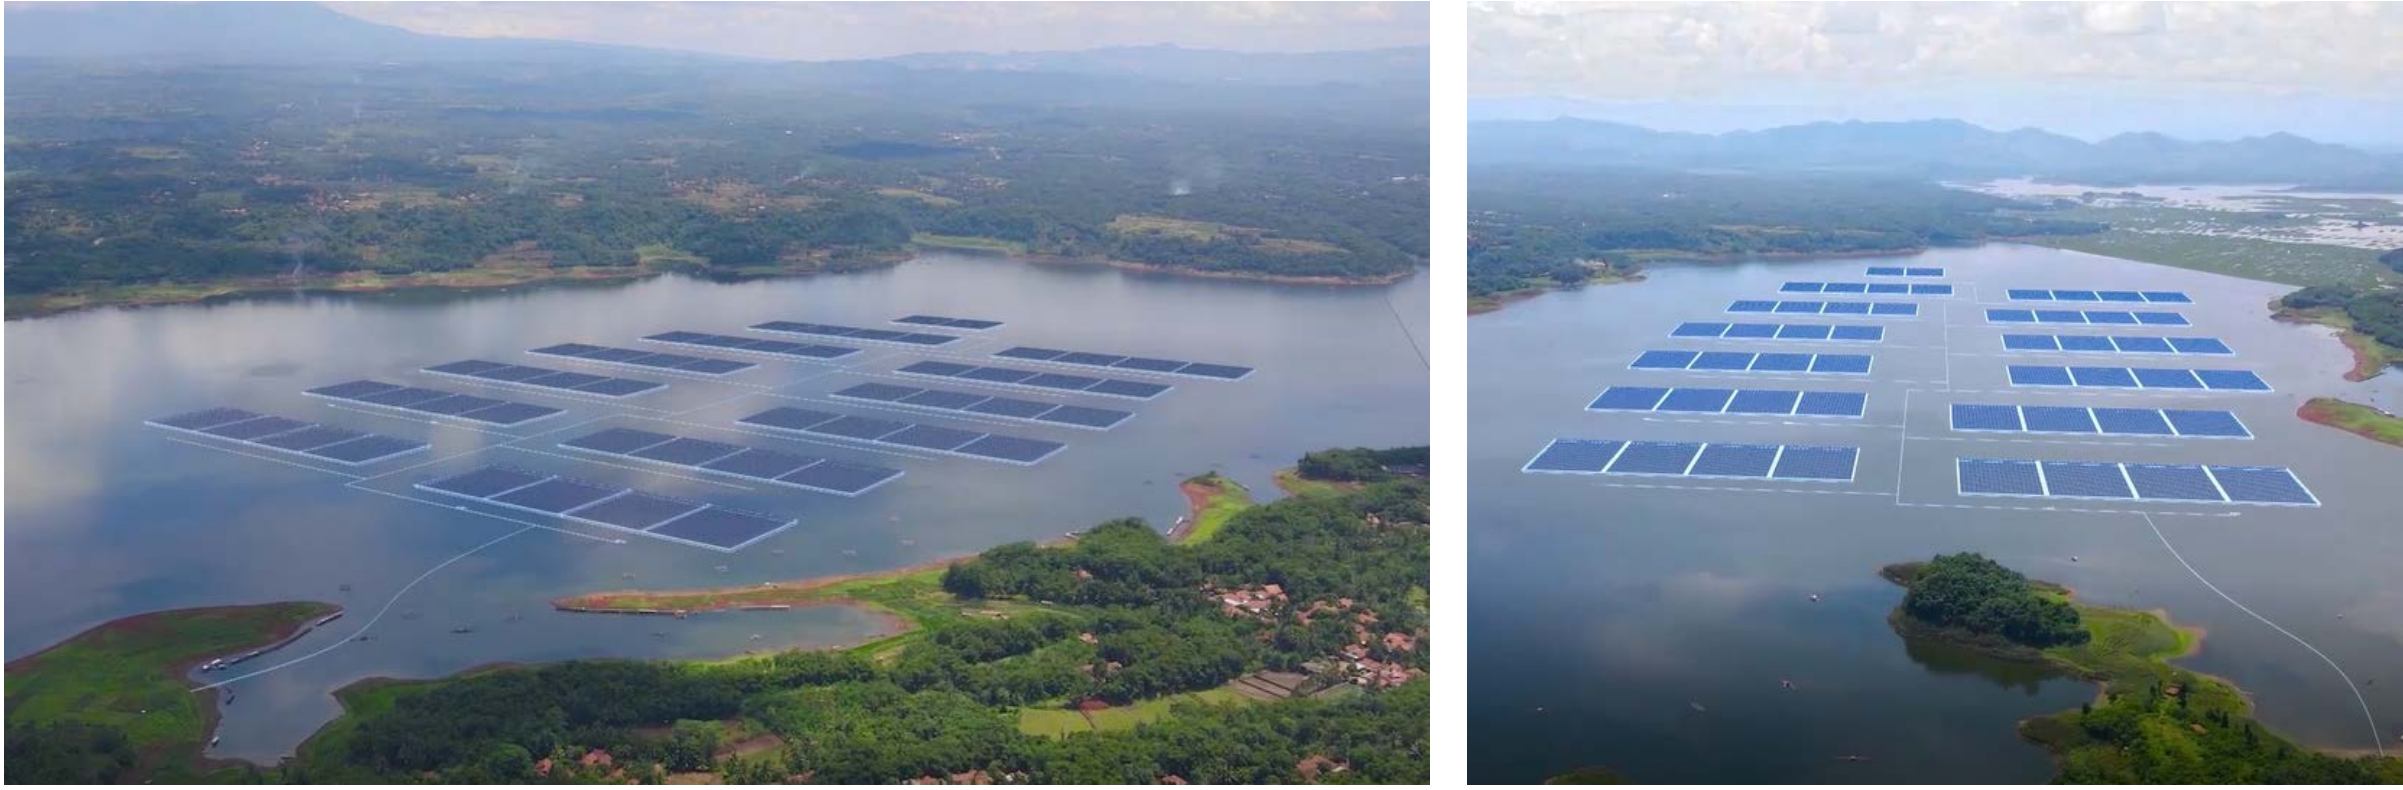
\includegraphics[width=0.86\textwidth]{fig_2_1_visualisasi_plts_cirata.png}
    \caption{Visualisasi PLTS Terapung Cirata pada area Waduk Cirata \cite{pmse2021}.}
    \label{gbr:visualisasi-plts-cirata}
    \vspace{-0.20cm}
\end{figure}

\section{Struktur Organisasi}
\label{sec:struktur-organisasi}

PLTS Terapung Cirata 145 MWac dimiliki dan dikelola oleh PT PMSE. PT PMSE merupakan perusahaan konsorsium atau \textit{joint venture} antara PT Pembangkitan Jawa Bali (PT PJB) dan Abu Dhabi Future Energy Company (Masdar). Komposisi kepemilikan saham terdiri atas 51\% oleh PT PJB dan 49\% oleh Masdar \cite{pmse2021}.

PT PJB merupakan anak perusahaan PT PLN (Persero), sedangkan Masdar merupakan anak usaha dari Mubadala Investment Company. Dengan susunan tersebut, proyek PLTS Terapung Cirata melibatkan pihak Indonesia melalui PLN dan PT PJB, serta pihak Uni Emirat Arab melalui Masdar. Struktur kepemilikan PT PMSE ditunjukkan pada Gambar~\ref{gbr:struktur-kepemilikan-pmse}.

\begin{figure}[H]
    \centering
    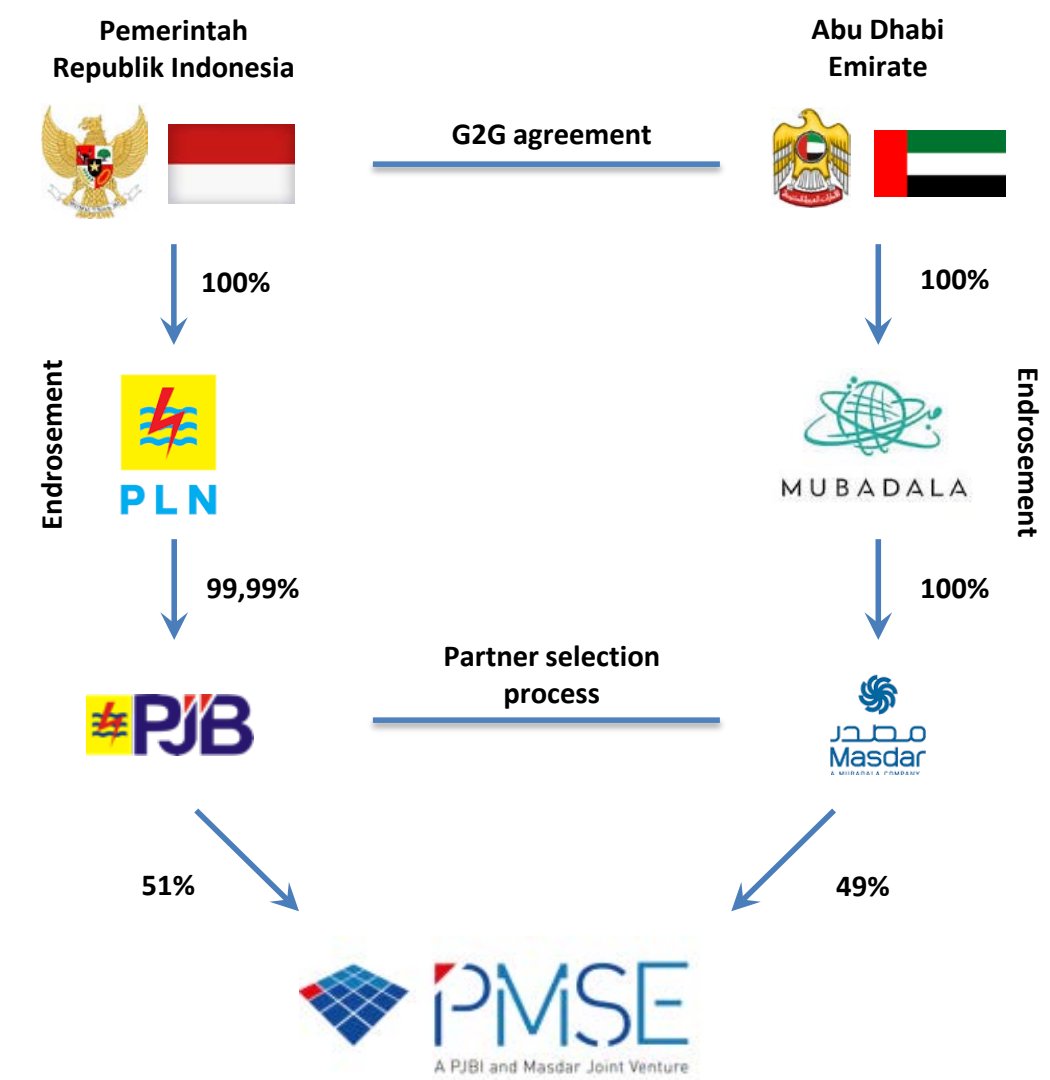
\includegraphics[width=0.62\textwidth]{fig_2_2_struktur_kepemilikan.png}
    \caption{Struktur kepemilikan PT PMSE \cite{pmse2021}.}
    \label{gbr:struktur-kepemilikan-pmse}
    \vspace{-0.20cm}
\end{figure}

Pada tingkat manajemen, struktur PT PMSE mencakup fungsi pimpinan perusahaan, operasi, serta keuangan dan administrasi. Pembagian fungsi tersebut diperlukan agar pengelolaan proyek, pelaksanaan operasi, dan administrasi perusahaan dapat berjalan secara terkoordinasi.

\section{Tugas dan Tanggung Jawab}
\label{sec:tugas-tanggung-jawab}

PT PMSE berperan sebagai pemilik dan pengelola proyek PLTS Terapung Cirata. Dalam skema PPA, tanggung jawab utama perusahaan mencakup penyediaan pembangkit, gardu induk, dan jalur transmisi 150 kV. Dengan demikian, peran PT PMSE tidak hanya terbatas pada pengelolaan pembangkit, tetapi juga mencakup penyiapan infrastruktur agar energi listrik yang dihasilkan dapat disalurkan ke sistem kelistrikan PLN.

Pelaksanaan proyek melibatkan beberapa pihak dengan lingkup pekerjaan yang berbeda. Power China Corporation Group ditunjuk sebagai kontraktor \textit{Engineering, Procurement, and Construction} (EPC) utama. PT Tractebel Indonesia berperan sebagai \textit{Project Management Consultant} (PMC) atau \textit{owner engineer}, sedangkan DNV GL berperan sebagai \textit{Lender Technical Advisor} yang memberikan laporan teknis kepada pihak pemberi pinjaman \cite{pmse2021}. Hubungan pihak-pihak tersebut ditunjukkan pada Gambar~\ref{gbr:struktur-proyek-plts-cirata}.

\begin{figure}[H]
    \centering
    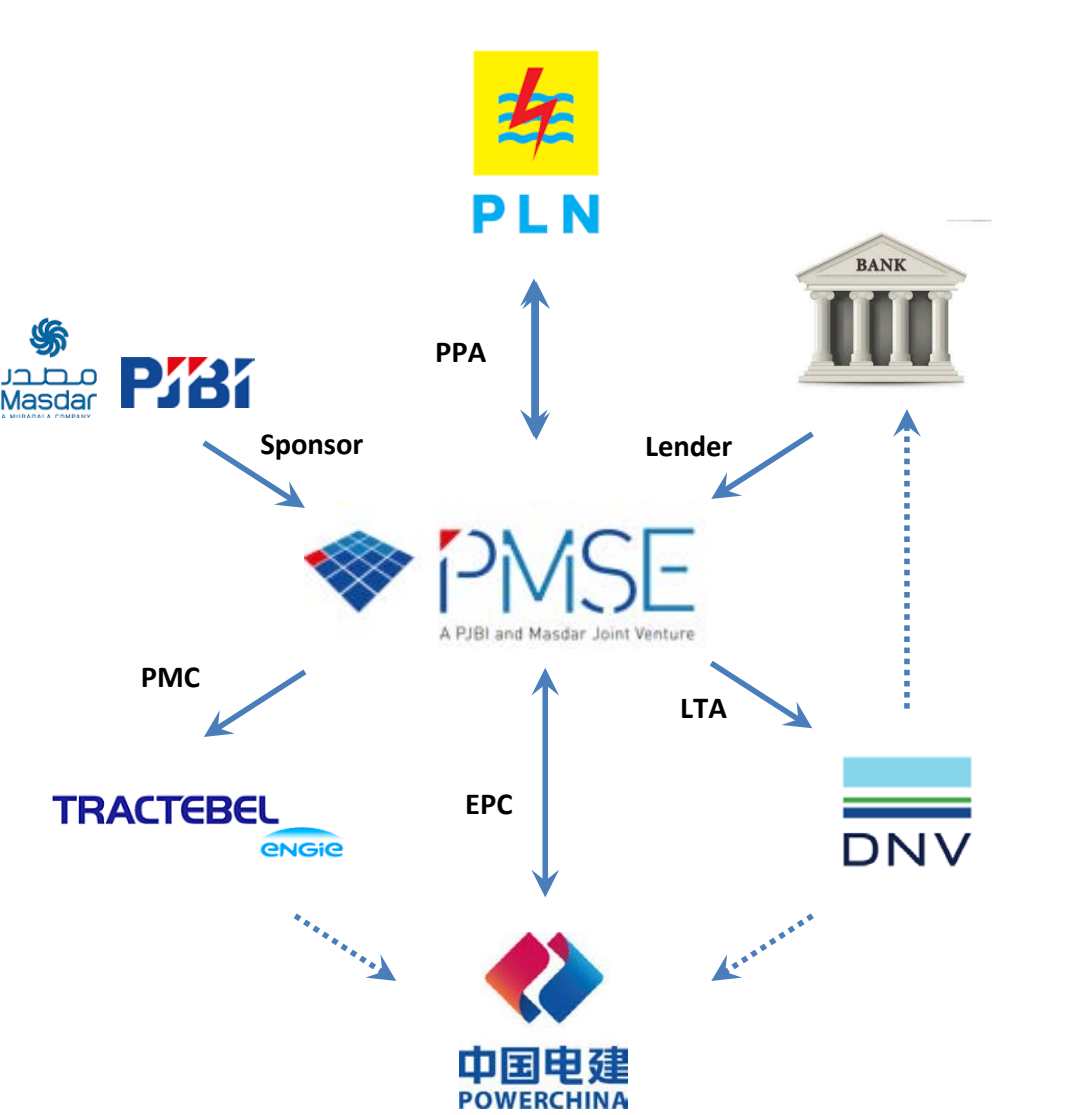
\includegraphics[width=0.62\textwidth]{fig_2_3_struktur_proyek.png}
    \caption{Struktur proyek PLTS Terapung Cirata \cite{pmse2021}.}
    \label{gbr:struktur-proyek-plts-cirata}
    \vspace{-0.20cm}
\end{figure}

Berdasarkan lingkup tersebut, tugas dan tanggung jawab umum PT PMSE pada proyek PLTS Terapung Cirata dapat dirangkum sebagai berikut.

\begin{packed_enum}
    \item Mengelola pengembangan dan pengoperasian proyek PLTS Terapung Cirata.
    \item Menyediakan pembangkit, gardu induk, dan jalur transmisi 150 kV sesuai lingkup PPA.
    \item Melakukan koordinasi dengan PLN, kontraktor EPC, konsultan manajemen proyek, dan penasihat teknis lender.
    \item Menjaga keberlanjutan operasi pembangkit melalui kegiatan inspeksi, pemeliharaan, dan evaluasi teknis.
\end{packed_enum}

Secara umum, tahapan pengembangan PLTS Terapung Cirata meliputi inisiasi, studi kelayakan, pengajuan proyek, pemilihan mitra, penyusunan PPA, pembentukan perusahaan proyek, pengurusan perizinan, pembiayaan, konstruksi, hingga operasi. Rangkaian tersebut menunjukkan bahwa proyek PLTS terapung memerlukan koordinasi lintas bidang, mulai dari aspek teknis, finansial, legal, perizinan, konstruksi, sampai operasi dan pemeliharaan.

Dari sisi teknis, sistem PLTS Terapung Cirata tersusun atas modul surya, sistem pelampung, DC combiner, inverter, transformator penaik tegangan, sistem \textit{anchoring} dan \textit{mooring}, serta jalur transmisi. Komponen-komponen tersebut bekerja secara terintegrasi untuk mengubah radiasi matahari menjadi energi listrik yang dapat disalurkan ke jaringan. Susunan komponen utama PLTS terapung ditunjukkan pada Gambar~\ref{gbr:teknologi-plts-terapung}.

\begin{figure}[H]
    \centering
    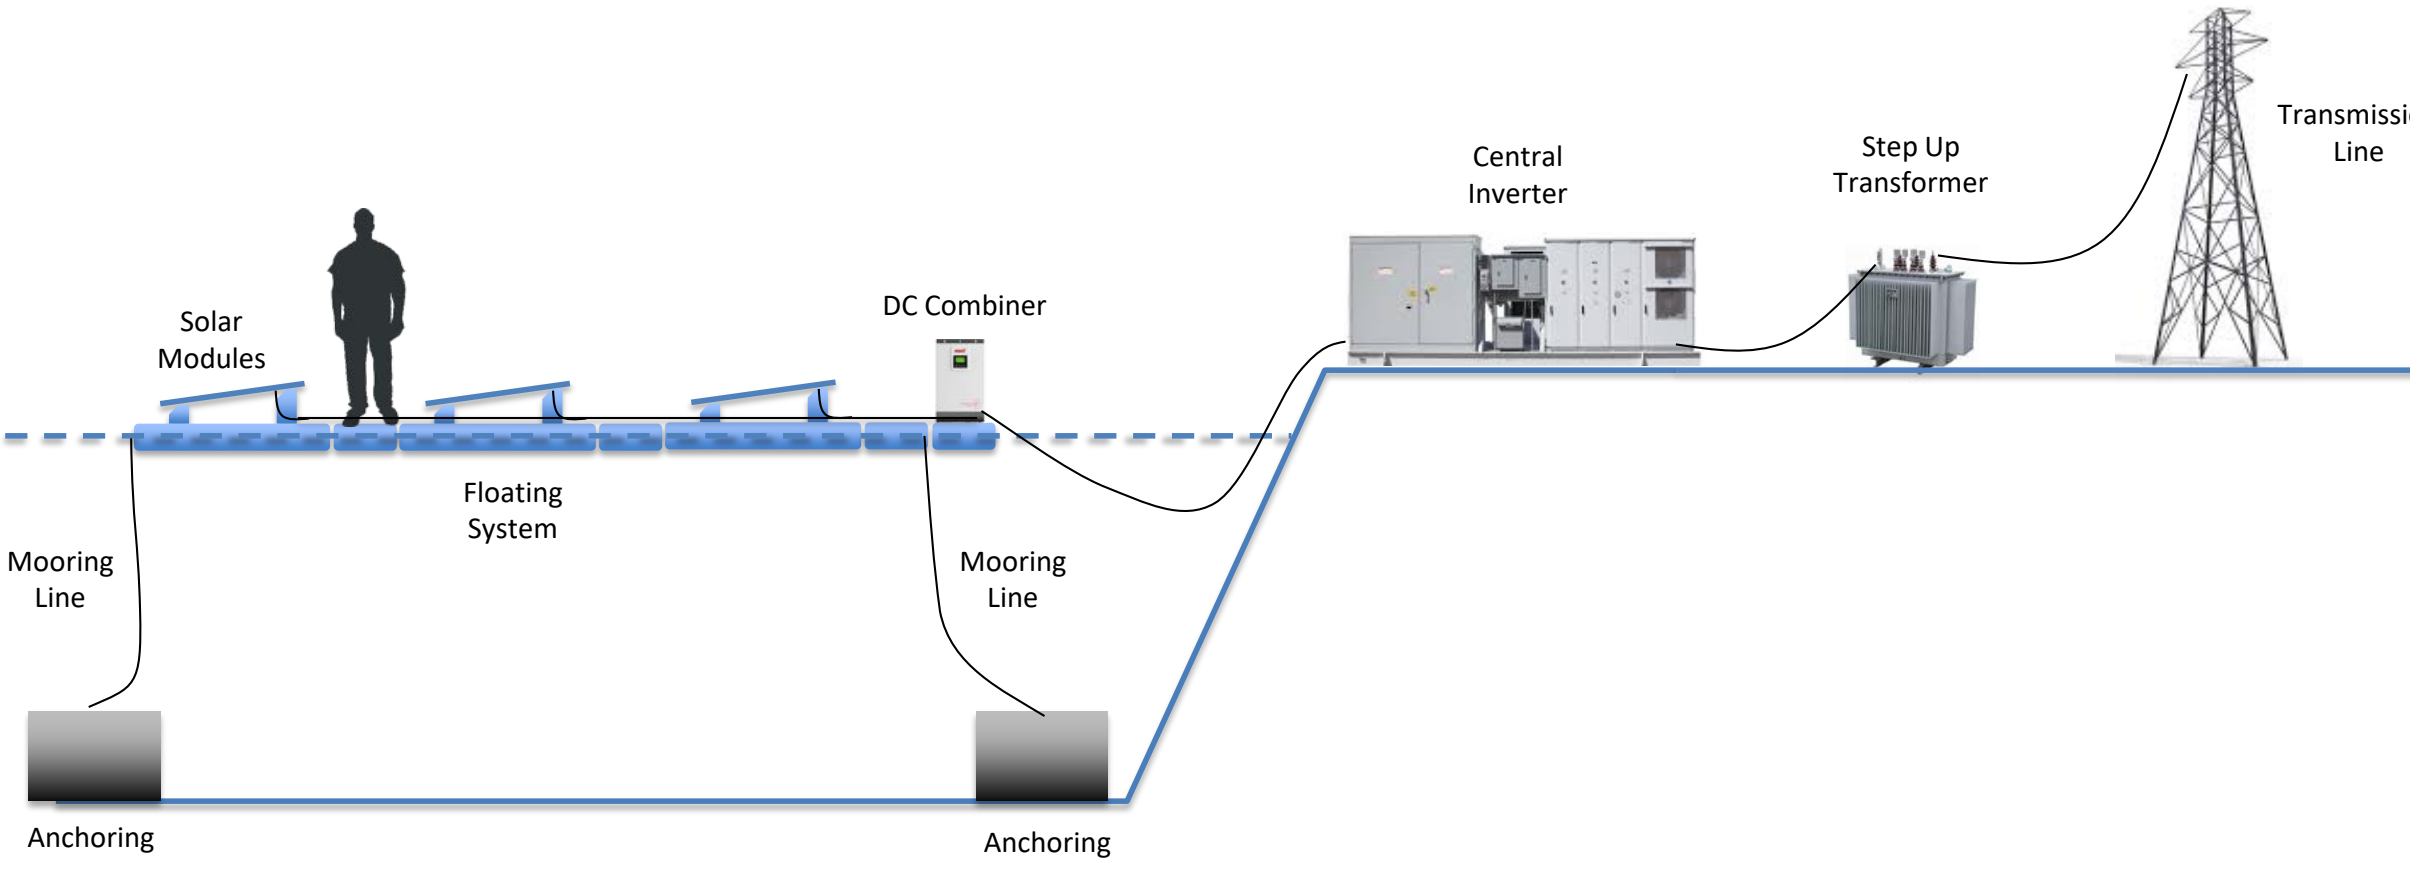
\includegraphics[width=0.86\textwidth]{fig_2_4_teknologi_plts_terapung.png}
    \caption{Komponen utama teknologi PLTS terapung \cite{pmse2021}.}
    \label{gbr:teknologi-plts-terapung}
    \vspace{-0.20cm}
\end{figure}

\section{Kesehatan dan Keselamatan Kerja (K3)}
\label{sec:k3}

Kegiatan kerja praktik di lingkungan PLTS Terapung Cirata memerlukan perhatian terhadap aspek kesehatan dan keselamatan kerja karena aktivitas dilakukan pada area pembangkit, area perairan, dan fasilitas kelistrikan. Penerapan K3 dilakukan dengan mengikuti arahan pembimbing lapangan, ketentuan perusahaan, serta instruksi HSE yang berlaku di lokasi. Penggunaan alat pelindung diri, pembatasan akses ke area tertentu, dan pendampingan ketika berada di area kerja menjadi bagian penting dalam pelaksanaan kegiatan lapangan. Rincian mengenai aspek-aspek K3 yang diterapkan selama kerja praktik tercantum pada Tabel~\ref{tab:k3-kerja-praktik}.

Sebelum melaksanakan aktivitas di area \textit{offshore} PLTS Terapung Cirata, mahasiswa kerja praktik terlebih dahulu mengikuti pengenalan keselamatan kerja. Kegiatan ini membahas aturan dasar K3, potensi bahaya di area pembangkit dan perairan, penggunaan alat pelindung diri, prosedur akses area kerja, serta mekanisme komunikasi dengan petugas lapangan. Dalam pelaksanaan kerja praktik, pengenalan K3 diberikan oleh HSE HDEC/PowerChina yang berada dalam lingkup kontraktor EPC proyek. Di sisi lain, PT PMSE sebagai pengelola PLTS Terapung Cirata juga memiliki fungsi HSE untuk memastikan kegiatan operasi dan pemeliharaan berjalan sesuai prosedur keselamatan. Kegiatan pengenalan K3 tersebut ditunjukkan pada Gambar~\ref{gbr:pengenalan-k3-hdec}.

\begin{figure}[H]
    \centering
    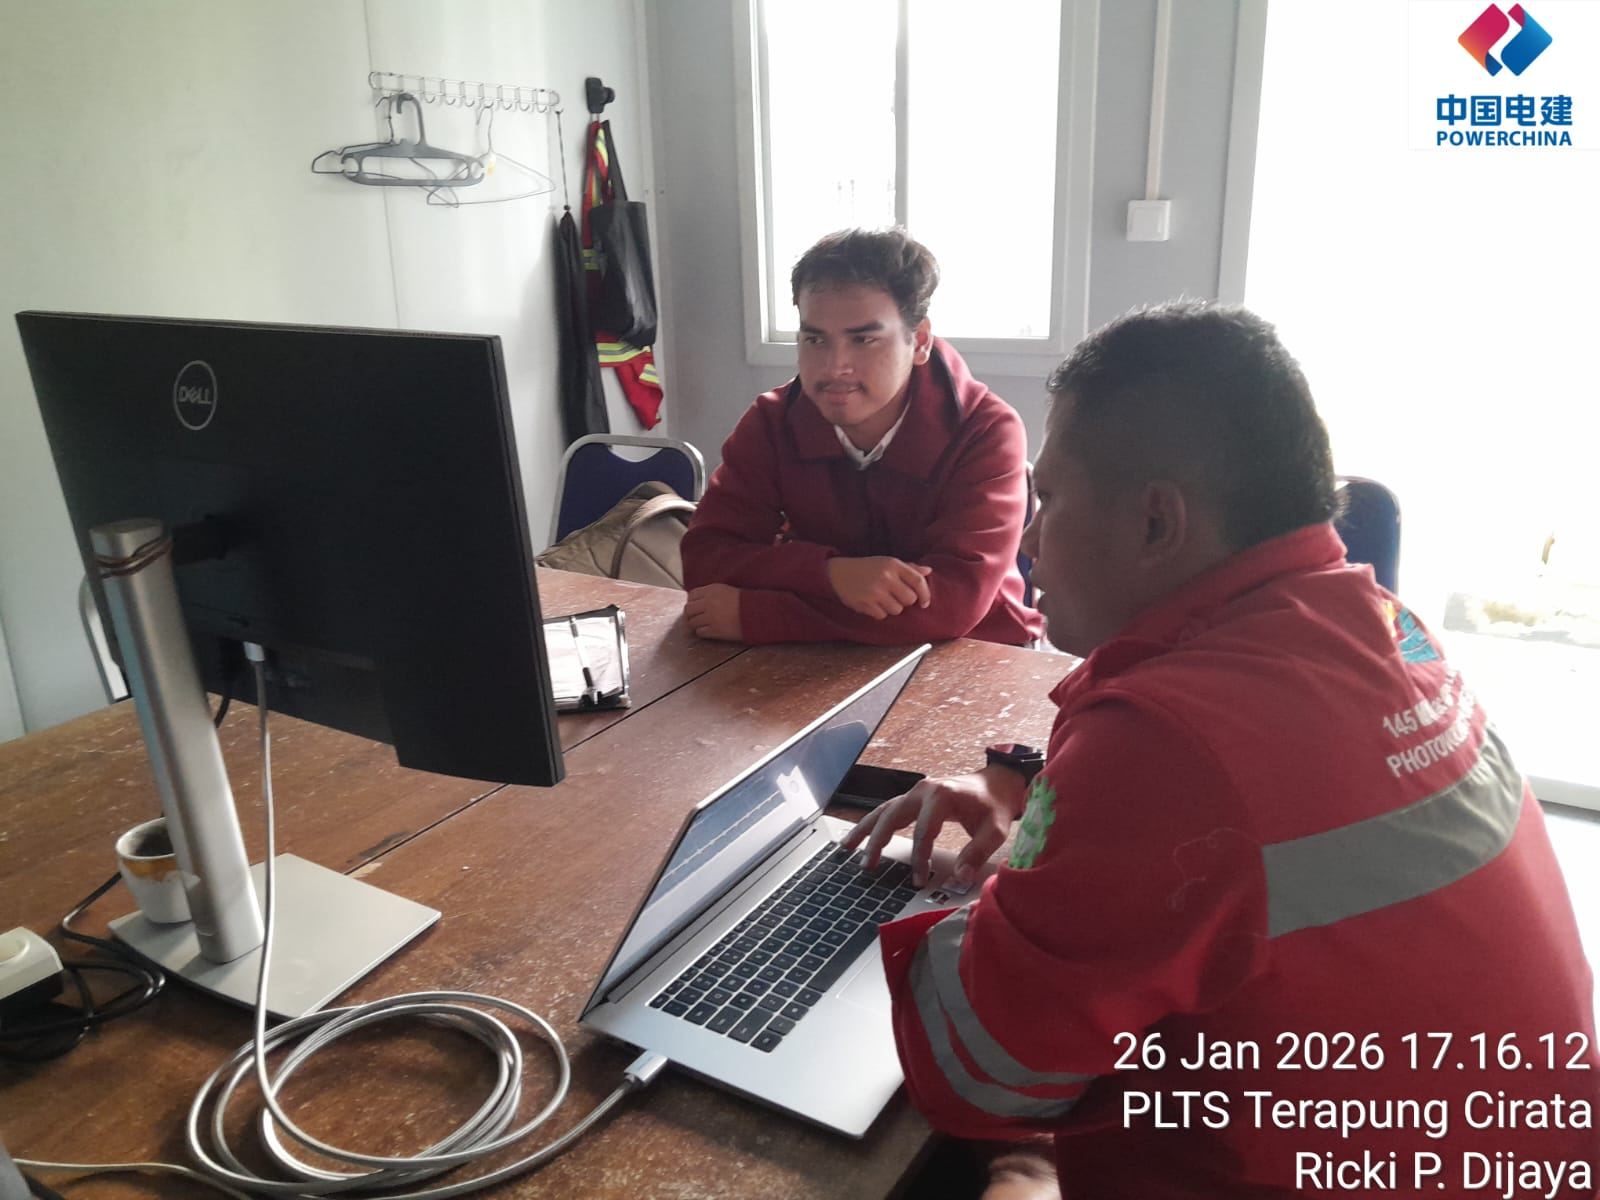
\includegraphics[width=0.86\textwidth]{fig_2_5_pengenalan_k3_hdec.jpeg}
    \caption{Pengenalan K3 sebelum kegiatan lapangan di PLTS Terapung Cirata.}
    \label{gbr:pengenalan-k3-hdec}
    \vspace{-0.20cm}
\end{figure}

Selain pengenalan K3, mahasiswa juga mengikuti kegiatan \textit{Basic Sea Survival} (BSS) sebagai pembekalan sebelum melakukan aktivitas pada area perairan. Kegiatan BSS diberikan untuk meningkatkan kesiapan peserta dalam menghadapi kondisi darurat di air, terutama karena sebagian area kerja PLTS Terapung Cirata berada di atas Waduk Cirata. Materi dan latihan yang diberikan meliputi pengenalan alat keselamatan, penggunaan pelampung, teknik mengapung, serta prosedur dasar penyelamatan diri ketika berada di perairan. Latihan Basic Sea Survival (BSS) mahasiswa ditunjukkan pada Gambar~\ref{gbr:basic-sea-survival}.

\begin{figure}[H]
    \centering
    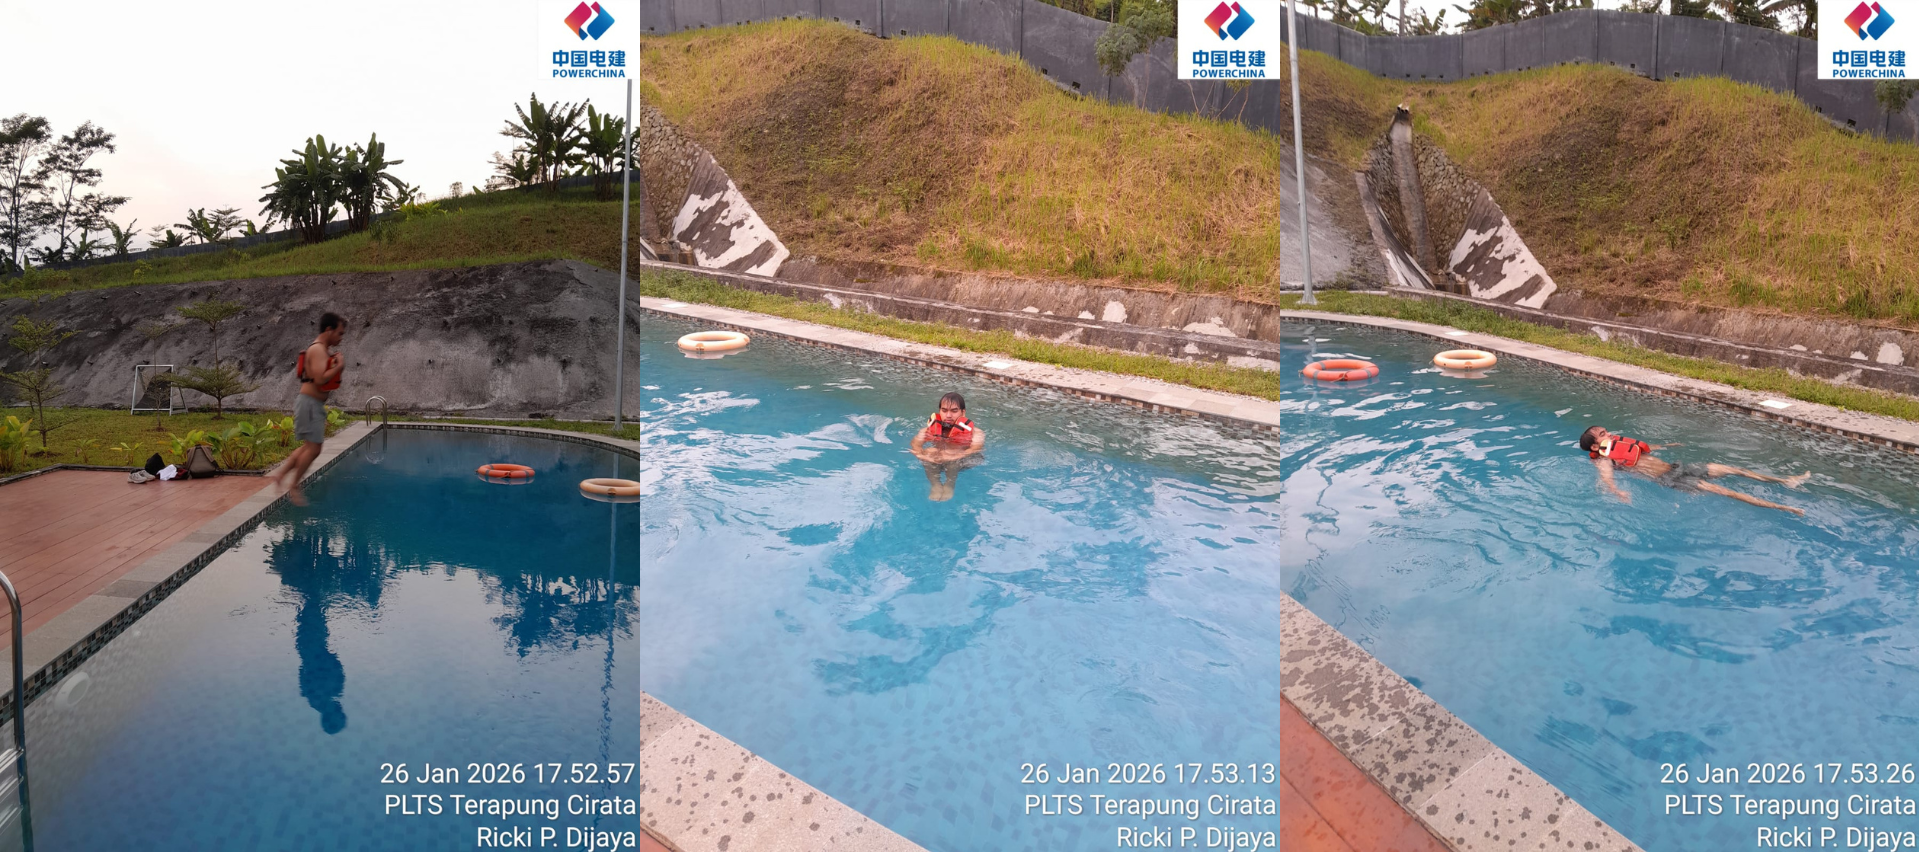
\includegraphics[width=0.92\textwidth]{fig_2_6_basic_sea_survival.png}
    \caption{Kegiatan \textit{Basic Sea Survival} sebelum aktivitas di area perairan.}
    \label{gbr:basic-sea-survival}
    \vspace{-0.20cm}
\end{figure}

\begin{table}[H]
    \centering
    \caption{Aspek K3 selama kerja praktik di PLTS Terapung Cirata}
    \label{tab:k3-kerja-praktik}
    \vspace{0.05cm}
    {\small
    \renewcommand{\arraystretch}{1.20}
    \begin{tabularx}{\textwidth}{
        >{\centering\arraybackslash}p{1.0cm}
        >{\raggedright\arraybackslash}p{4.0cm}
        >{\raggedright\arraybackslash}X
    }
        \toprule
        \textbf{No.} & \textbf{Nama} & \textbf{Fungsi} \\
        \midrule
        1 & \textit{Pengenalan K3} & Memberikan pemahaman mengenai aturan keselamatan, potensi bahaya, penggunaan APD, dan prosedur akses area kerja. \\
        \midrule
        2 & \textit{Basic Sea Survival} & Membekali peserta dengan kemampuan dasar keselamatan di perairan sebelum aktivitas \textit{offshore}. \\
        \midrule
        3 & \textit{Alat Pelindung Diri} & Mengurangi risiko kecelakaan melalui penggunaan helm keselamatan, sepatu keselamatan, rompi, dan pelampung sesuai kebutuhan area kerja. \\
        \midrule
        4 & \textit{Pendampingan Lapangan} & Memastikan kegiatan mahasiswa dilakukan sesuai batas kewenangan, arahan pembimbing, dan prosedur keselamatan di lokasi. \\
        \bottomrule
    \end{tabularx}}
    \vspace{-0.15cm}
\end{table}

Pada sisi operasi dan pemeliharaan, PLTS Terapung Cirata memiliki jalur \textit{gangway} sebagai akses teknisi. Akses menuju \textit{array} dilakukan ketika terdapat kegiatan inspeksi, perbaikan, penggantian komponen, atau pemeriksaan visual secara detail. Selama kerja praktik, aktivitas lapangan dilakukan dengan memperhatikan batas kewenangan mahasiswa, arahan pembimbing, dan prosedur keselamatan yang berlaku di lokasi. Akses inspeksi dan pemeliharaan pada PLTS terapung ditunjukkan pada Gambar~\ref{gbr:pemeliharaan-plts-terapung}.

\begin{figure}[H]
    \centering
    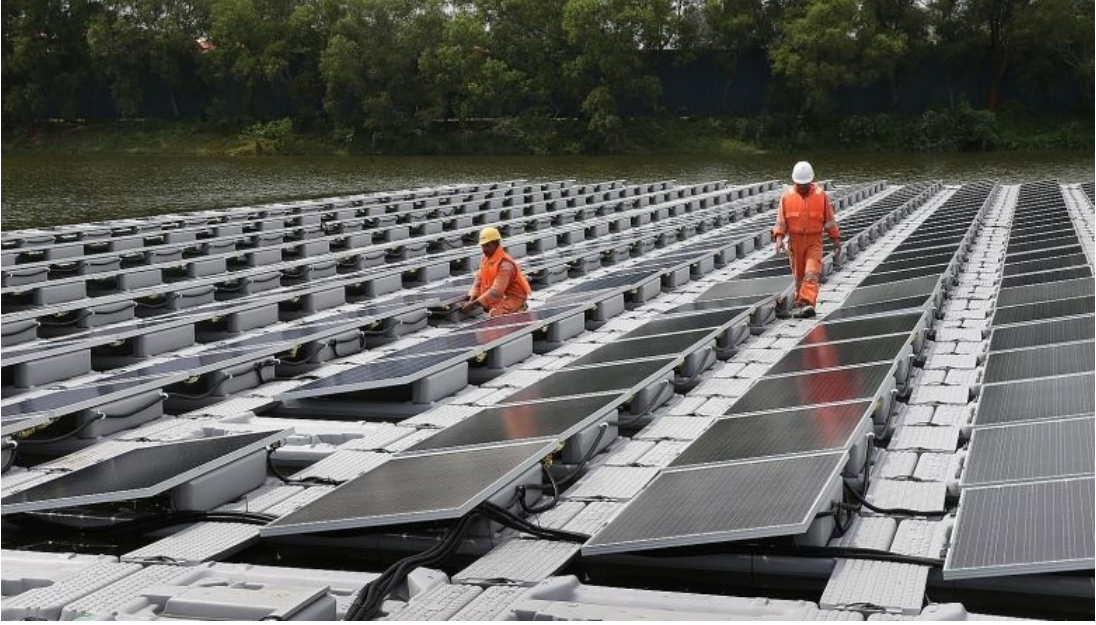
\includegraphics[width=0.78\textwidth]{fig_2_6_proses_pemeliharaan.png}
    \caption{Kegiatan inspeksi dan pemeliharaan pada PLTS terapung \cite{pmse2021}.}
    \label{gbr:pemeliharaan-plts-terapung}
    \vspace{-0.20cm}
\end{figure}

\section{Etika Profesi}
\label{sec:etika-profesi}

Etika profesi selama kerja praktik diterapkan melalui kedisiplinan, tanggung jawab, dan kepatuhan terhadap arahan pembimbing lapangan. Mahasiswa perlu menjaga perilaku profesional di lingkungan kerja, menghormati aturan perusahaan, serta menggunakan waktu kerja praktik untuk memperoleh pemahaman teknis secara aktif dan bertanggung jawab.

Mahasiswa juga perlu menjaga kerahasiaan data dan informasi yang diperoleh selama kegiatan kerja praktik, terutama informasi teknis, dokumentasi internal, dan data proyek yang tidak diperkenankan untuk disebarluaskan. Penggunaan dokumentasi, foto, maupun data pengukuran dilakukan dengan memperhatikan izin dari pihak yang berwenang.

Dalam penyusunan laporan, etika profesi diwujudkan melalui kejujuran dalam pengolahan data, ketelitian dalam penulisan, serta pencantuman sumber informasi yang digunakan. Dengan demikian, laporan kerja praktik tidak hanya menjadi dokumentasi kegiatan, tetapi juga menjadi bentuk pertanggungjawaban akademik dan profesional mahasiswa teknik elektro.

% !TEX root = ../main.tex
% =========================================================
% bab3.tex - POKOK PEMBAHASAN
% Dasar teori dan metodologi teknis analisis modul PV
% pasca-terendam.
% Memerlukan tambahan paket: amssymb, booktabs, circuitikz,
% pgfplots, dan pustaka tikz (lihat preambles_tambahan.tex).
% =========================================================

\chapter[POKOK PEMBAHASAN]{\\ POKOK PEMBAHASAN}

Bab ini membahas dasar teori dan metodologi teknis yang digunakan dalam
analisis kelayakan modul PV pasca-terendam pada PLTS Terapung Cirata.
Pembahasan dimulai dari gambaran umum sistem PLTS terapung, konfigurasi
modul-\textit{string}-\textit{array}, karakteristik kurva I--V dan P--V,
parameter elektrikal modul, Fill Factor dan indikator arus--tegangan,
representasi mekanisme \textit{fault} pada level sistem, serta objek dan
tahapan pengolahan data.

\section{Gambaran Umum Sistem PLTS Terapung}

PLTS terapung merupakan sistem pembangkit listrik tenaga surya yang dipasang di
atas struktur apung pada permukaan air. Secara umum, sistem ini terdiri dari
modul PV, struktur apung, sistem \textit{mooring} dan \textit{anchoring},
\textit{DC combiner}, inverter, transformator, sistem proteksi, dan saluran
transmisi. Gambaran umum sistem PLTS terapung ditunjukkan pada
Gambar~\ref{gbr:sistem-umum-plts-terapung}.

\begin{figure}[H]
\centering
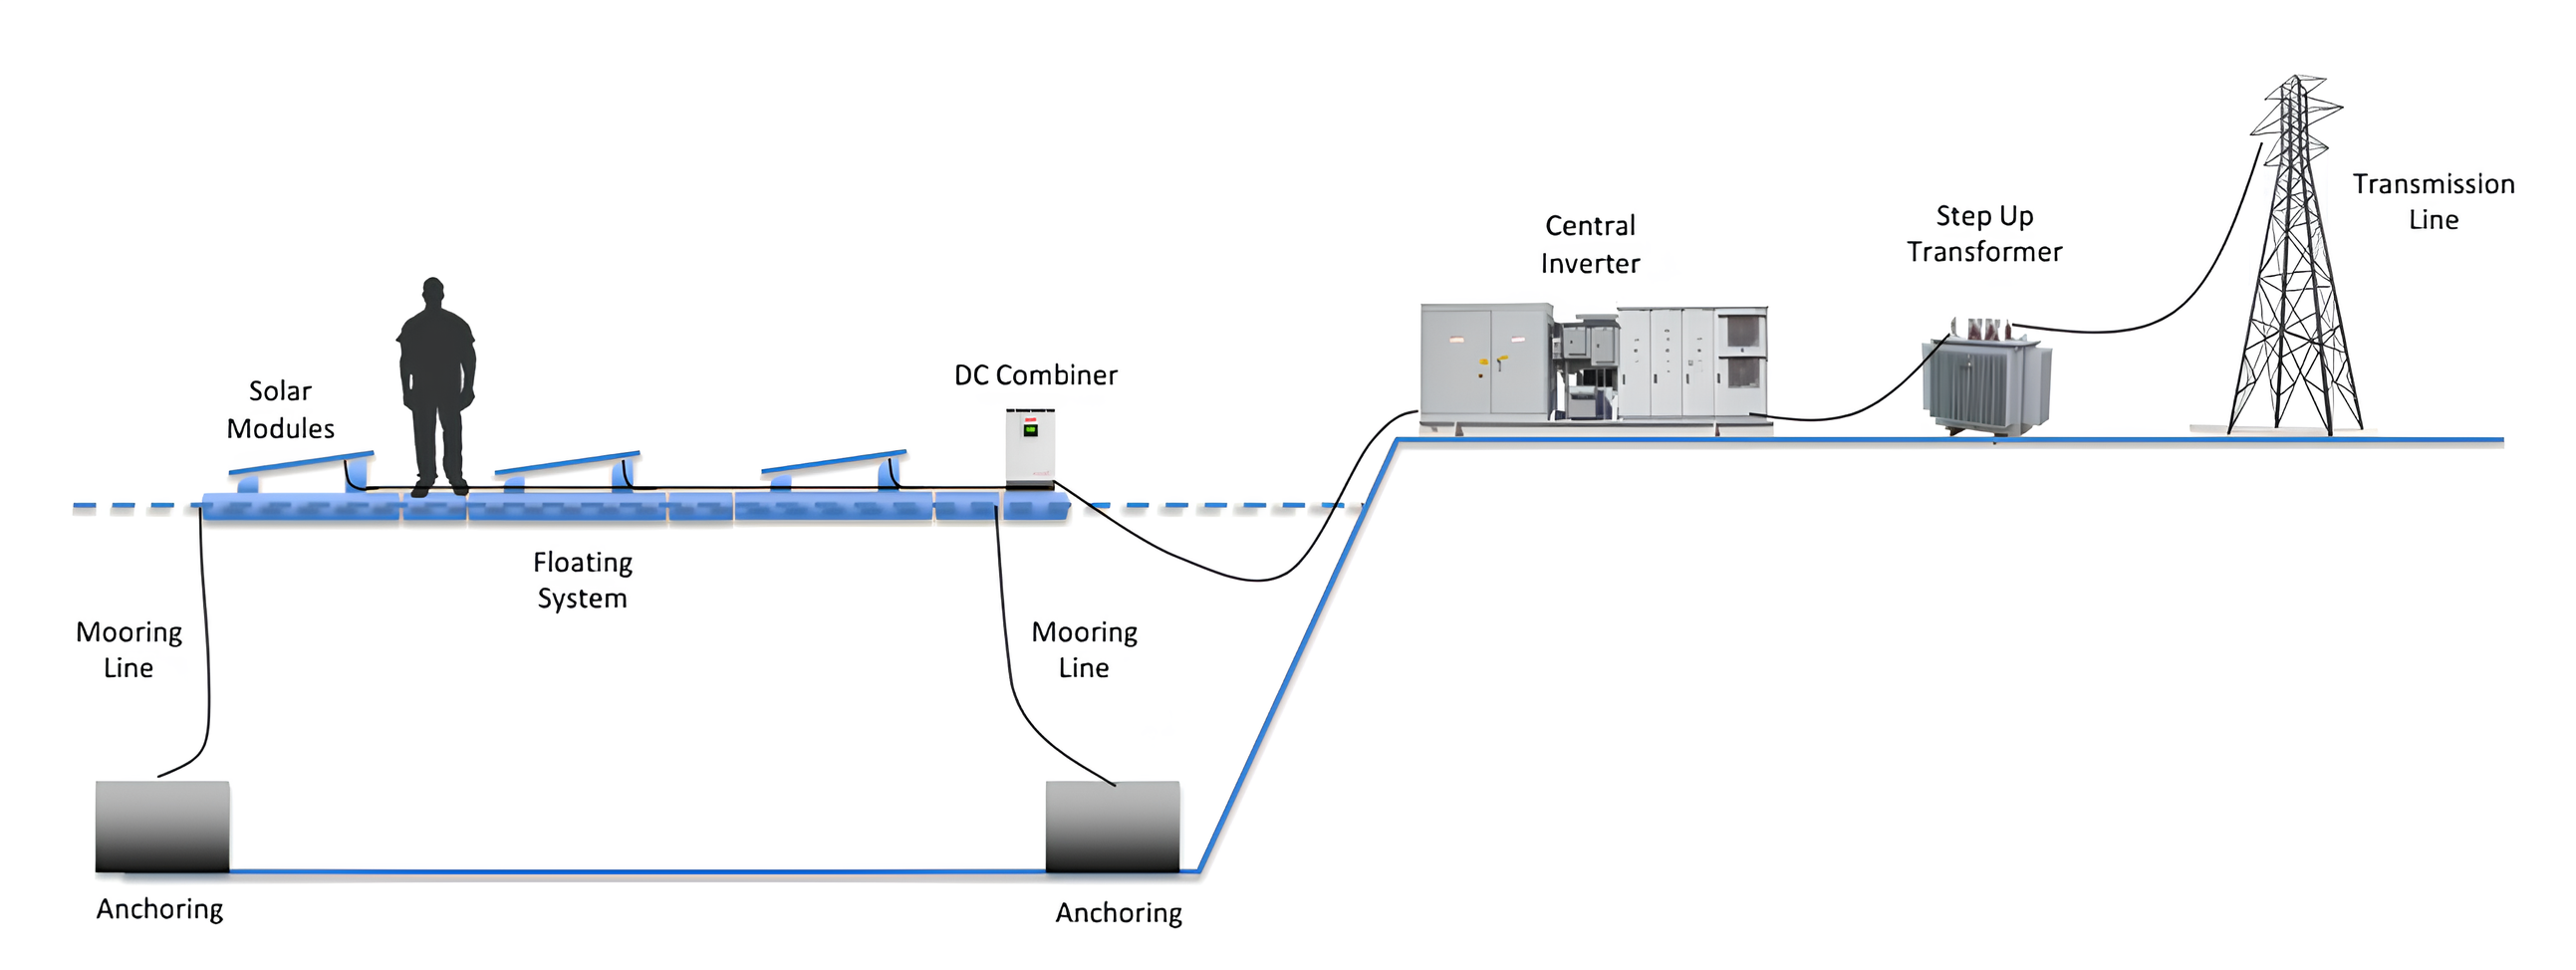
\includegraphics[width=0.80\textwidth]{sistem-umum-plts-terapung.png}
\caption{Sistem umum PLTS terapung.}
\label{gbr:sistem-umum-plts-terapung}
\end{figure}

Pada Gambar~\ref{gbr:sistem-umum-plts-terapung}, modul PV berfungsi mengubah
energi radiasi matahari menjadi energi listrik DC. Energi listrik dari beberapa
modul dikumpulkan melalui \textit{DC combiner}, kemudian disalurkan ke inverter
untuk dikonversi menjadi energi listrik AC. Tegangan keluaran inverter
selanjutnya dinaikkan melalui transformator sebelum disalurkan ke jaringan.
Selain komponen elektrik, sistem PLTS terapung juga memerlukan struktur apung,
\textit{mooring}, dan \textit{anchoring} untuk menjaga posisi instalasi pada
permukaan air \cite{worldbankFPV2019,ieaFPV2025}.

Perbedaan utama PLTS terapung dibandingkan PLTS berbasis darat terletak pada
lingkungan operasinya. Modul PV, kabel, konektor, dan struktur pendukung berada
pada lingkungan yang dipengaruhi oleh air, kelembapan, perubahan muka air, dan
pergerakan struktur apung. Kondisi tersebut menjadi relevan dalam laporan ini
karena modul PV pasca-terendam perlu dievaluasi melalui parameter elektrik
sebelum keputusan operasional diambil.

\section{Modul PV, String, dan Array}

Modul PV merupakan unit dasar pada sistem PLTS yang menghasilkan daya listrik
DC dari radiasi matahari. Dalam sistem PLTS, modul PV tidak bekerja sebagai
komponen tunggal. Beberapa modul dihubungkan secara seri membentuk satu
\textit{string}. Pada hubungan seri, arus yang mengalir pada setiap modul
bernilai sama, sedangkan tegangan \textit{string} merupakan penjumlahan
tegangan dari seluruh modul yang berada dalam \textit{string} tersebut. Oleh
karena itu, perubahan karakteristik pada salah satu modul dapat memengaruhi
titik kerja \textit{string}, terutama apabila modul tersebut mengalami
penurunan tegangan operasi atau tidak mampu mengikuti arus operasi modul
lainnya.

Beberapa \textit{string} kemudian dihubungkan secara paralel membentuk
\textit{array}. Pada hubungan paralel, tegangan antar \textit{string} relatif
sama karena terhubung pada bus DC yang sama, sedangkan arus \textit{array}
merupakan penjumlahan arus dari setiap \textit{string}. Dengan konfigurasi ini,
daya total sistem PV bergantung pada kontribusi tegangan setiap modul dalam
\textit{string} dan kontribusi arus setiap \textit{string} dalam
\textit{array}. Konfigurasi modul, \textit{string}, dan \textit{array}
ditunjukkan pada Gambar~\ref{gbr:array_config}.

\begin{figure}[H]
\centering
\begin{tikzpicture}[x=1cm,y=1cm,>=Latex,font=\scriptsize]
\node[pvmod] (m11) at (0,2.4) {PV};
\node[pvmod] (m12) at (1,2.4) {PV};
\node[lab] (d1) at (1.85,2.4) {$\cdots$};
\node[pvmod] (m1n) at (2.7,2.4) {PV};
\node[lab] at (1.35,3.0) {String 1};

\node[pvmod] (m21) at (0,1.4) {PV};
\node[pvmod] (m22) at (1,1.4) {PV};
\node[lab] (d2) at (1.85,1.4) {$\cdots$};
\node[pvmod] (m2n) at (2.7,1.4) {PV};

\node[pvmod] (m31) at (0,0.4) {PV};
\node[pvmod] (m32) at (1,0.4) {PV};
\node[lab] (d3) at (1.85,0.4) {$\cdots$};
\node[pvmod] (m3n) at (2.7,0.4) {PV};
\node[lab] at (1.35,-0.2) {String $N_P$};

\draw[line width=0.6pt] (m11) -- (m12) -- (d1) -- (m1n);
\draw[line width=0.6pt] (m21) -- (m22) -- (d2) -- (m2n);
\draw[line width=0.6pt] (m31) -- (m32) -- (d3) -- (m3n);

\draw[line width=0.7pt] (3.15,0.4) -- (3.5,0.4);
\draw[line width=0.7pt] (3.15,1.4) -- (3.5,1.4);
\draw[line width=0.7pt] (3.15,2.4) -- (3.5,2.4);
\draw[line width=0.7pt] (3.5,0.4) -- (3.5,2.4);
\draw[line width=0.7pt] (3.5,1.4) -- (5,1.4);

\node[draw, rectangle, minimum width=1.2cm, minimum height=0.8cm, line width=0.6pt, font=\scriptsize] (cb) at (5.8,1.4) {DC Combiner};
\draw[line width=0.7pt] (cb.east) -- (7.5,1.4);
\node[draw, rectangle, minimum width=1.2cm, minimum height=0.8cm, line width=0.6pt, font=\scriptsize] (inv) at (8.3,1.4) {Inverter};

\node[lab] at (4.35,1.75) {Bus DC};
\node[lab] at (1.35,1.0) {$\vdots$};

% Penanda array: hanya mencakup kumpulan string dan bus paralel sebelum DC Combiner
\draw[dashed, rounded corners=4pt, line width=0.8pt]
(-0.85,-0.55) rectangle (3.85,3.25);

\node[lab, fill=white, inner sep=1pt] at (3.20,3.25) {Array};

\end{tikzpicture}
\caption{Konfigurasi modul, \textit{string}, dan \textit{array} pada sistem PV.}
\label{gbr:array_config}
\end{figure}

Pada konfigurasi seri, tegangan \textit{string} dapat dinyatakan sebagai
penjumlahan tegangan setiap modul, seperti ditunjukkan pada
persamaan~\eqref{eq:vstring}.
\begin{equation}
V_{string} = \sum_{j=1}^{N_s} V_{mod,j}
\label{eq:vstring}
\end{equation}

Pada konfigurasi paralel, arus \textit{array} merupakan penjumlahan arus dari
setiap \textit{string}, seperti ditunjukkan pada persamaan~\eqref{eq:iarray}.
\begin{equation}
I_{array} = \sum_{k=1}^{N_P} I_{string,k}
\label{eq:iarray}
\end{equation}

Persamaan~\eqref{eq:vstring} dan \eqref{eq:iarray} menunjukkan bahwa gangguan
pada level modul dapat memengaruhi karakteristik elektrik pada level
\textit{string} maupun \textit{array}. Oleh karena itu, hubungan antara modul,
\textit{string}, dan \textit{array} perlu dipahami sebelum membahas perubahan
parameter listrik akibat kondisi modul PV pasca-terendam.

\section{Karakteristik Kurva I--V dan P--V Modul PV}

Sel surya dapat dimodelkan sebagai rangkaian ekuivalen dengan satu dioda
\cite{pei2019,villalva2009}. Rangkaian ekuivalen ini terdiri dari sumber arus
foton ($I_{PH}$), dioda paralel, resistansi seri ($R_s$), dan resistansi shunt
($R_{sh}$). Rangkaian ekuivalen tersebut ditunjukkan pada
Gambar~\ref{gbr:singlediode}.

\begin{figure}[H]
\centering
\begin{circuitikz}[scale=0.85, transform shape, font=\scriptsize]
\draw (0,0) to[american current source, l=$I_{PH}$, invert] (0,3);
\draw (0,3) -- (2,3);
\draw (2,3) to[D, l_=$D$] (2,0);
\draw (2,0) -- (0,0);
\draw (2,3) -- (3.5,3);
\draw (3.5,3) to[R, l_=$R_{sh}$] (3.5,0);
\draw (2,0) -- (3.5,0);
\draw (3.5,3) -- (5,3);
\draw (5,3) to[R, l=$R_s$] (7,3);
\draw (3.5,0) -- (7,0);
\draw (7,3) to[short, -o] (7.5,3);
\draw (7,0) to[short, -o] (7.5,0);

\node[font=\scriptsize] at (8.0,1.5) {$V$};
\draw[->] (7.7,2.7) -- (7.7,0.3);

% Panah arus dibuat lebih tinggi agar tidak bertabrakan dengan R_s
\node[font=\scriptsize] at (6.15,3.85) {$I$};
\draw[->] (5.55,3.65) -- (6.75,3.65);

\end{circuitikz}
\caption{Rangkaian ekuivalen sel surya berbasis model satu dioda.}
\label{gbr:singlediode}
\end{figure}
Persamaan arus--tegangan untuk satu sel surya berdasarkan rangkaian ekuivalen
pada Gambar~\ref{gbr:singlediode} ditunjukkan pada
persamaan~\eqref{eq:iv_cell} \cite{villalva2009}.
\begin{equation}
I = I_{PH} - I_0\left[\exp\left(\frac{q(V+IR_s)}{akT}\right) - 1\right]
    - \frac{V+IR_s}{R_{sh}}
\label{eq:iv_cell}
\end{equation}

Pada persamaan~\eqref{eq:iv_cell}, $I_0$ adalah arus saturasi balik dioda, $a$
adalah faktor idealitas dioda, $T$ adalah temperatur sel, $q$ adalah muatan
elektron, dan $k$ adalah konstanta Boltzmann. Modul PV pada umumnya terdiri
dari beberapa sel surya yang tersusun seri sehingga karakteristik I--V modul
mengikuti bentuk yang sama dengan sel tunggal, tetapi dengan $V_{oc}$ yang
lebih tinggi. Ilustrasi parameter penting pada kurva I--V modul ditunjukkan
pada Gambar~\ref{gbr:iv_param}.

\begin{figure}[H]
\centering
\begin{tikzpicture}
\begin{axis}[
    width=0.82\linewidth,
    height=0.32\textheight,
    xmin=0, xmax=55,
    ymin=0, ymax=15,
    xlabel={Tegangan (V)},
    ylabel={Arus (A)},
    grid=both,
    minor tick num=1,
    xtick={0,5,10,15,20,25,30,35,40,45,50,55},
    ytick={0,2,4,6,8,10,12,14},
    legend style={font=\scriptsize, at={(0.02,0.02)}, anchor=south west},
    clip=false,
    name=myplot,
]

%--- Kurva I--V ---
\addplot[blue, thick, no marks, smooth] coordinates {
    (0,  14.13) (5,  14.10) (10, 14.05) (15, 13.95) (20, 13.85)
    (25, 13.70) (30, 13.55) (35, 13.40) (38, 13.30) (40, 13.25)
    (41.95, 13.35) (43, 13.05) (45, 11.5)  (47,  9.0)
    (48,   6.5)  (49,  4.0)  (50,  1.8)  (50.5, 0.7) (50.67, 0)
};
\addlegendentry{Kurva I--V}

%--- Garis putus-putus vertikal: Vmp ---
\addplot[red!70, dashed, thin, no marks]
    coordinates {(41.95, 0) (41.95, 13.35)};

%--- Garis putus-putus vertikal: Voc ---
\addplot[red!70, dashed, thin, no marks]
    coordinates {(50.67, 0) (50.67, 13.35)};

%--- Garis putus-putus horizontal: Imp ---
\addplot[red!70, dashed, thin, no marks]
    coordinates {(0, 13.35) (41.95, 13.35)};

%--- Garis putus-putus horizontal: Isc ---
\addplot[red!70, dashed, thin, no marks]
    coordinates {(0, 14.13) (50.67, 14.13)};

%--- Titik MPP ---
\node[circle, fill=black, inner sep=2pt] at (axis cs:41.95, 13.35) {};
\node[font=\scriptsize, anchor=south west] at (axis cs:41.95, 13.35) {MPP};

%--- Titik Isc ---
\node[circle, fill=black, inner sep=2pt] at (axis cs:0, 14.13) {};

%--- Titik Voc ---
\node[circle, fill=black, inner sep=2pt] at (axis cs:50.67, 0) {};

%--- Label di sisi KANAN: Isc dan Imp ---
\node[font=\scriptsize, anchor=west] at (axis cs:55, 14.13) {$I_{sc}$};
\node[font=\scriptsize, anchor=west] at (axis cs:55, 13.35) {$I_{mp}$};

%--- Label di sisi ATAS: Vmp dan Voc ---
\node[font=\scriptsize, anchor=south] at (axis cs:41.95, 15) {$V_{mp}$};
\node[font=\scriptsize, anchor=south] at (axis cs:50.67, 15) {$V_{oc}$};

\end{axis}
\end{tikzpicture}
\caption{Parameter kelistrikan pada kurva I--V modul PV.}
\label{gbr:iv_param}
\end{figure}

\section{Parameter Elektrikal Modul PV}

Kurva I--V modul PV mengandung beberapa parameter penting yang
merepresentasikan kinerja modul, yaitu \textit{open-circuit voltage}
($V_{oc}$), \textit{short-circuit current} ($I_{sc}$), tegangan dan arus pada
titik daya maksimum ($V_{mp}$ dan $I_{mp}$), serta daya maksimum ($P_{max}$).
Daya maksimum modul didefinisikan sebagai hasil perkalian $V_{mp}$ dan
$I_{mp}$, seperti pada persamaan~\eqref{eq:pmax}.
\begin{equation}
P_{max} = V_{mp} \cdot I_{mp}
\label{eq:pmax}
\end{equation}

Parameter terukur dibandingkan dengan nilai \textit{nameplate} pada
\textit{datasheet} untuk mengevaluasi tingkat degradasi modul. Penurunan
$P_{max}$ menunjukkan berkurangnya kemampuan daya modul, sedangkan pola
penurunan pada $V_{oc}$, $I_{sc}$, $V_{mp}$, atau $I_{mp}$ memberikan petunjuk
awal mengenai sisi parameter yang paling terpengaruh.

\section{Fill Factor dan Indikator Arus--Tegangan}

Bentuk kurva I--V dinyatakan secara kuantitatif melalui Fill Factor ($FF$),
yaitu rasio antara daya maksimum aktual dengan daya maksimum ideal yang
dihitung dari $V_{oc}$ dan $I_{sc}$, seperti pada
persamaan~\eqref{eq:ff} \cite{linwu2025}.
\begin{equation}
FF = \frac{P_{max}}{V_{oc} \cdot I_{sc}}
   = \frac{V_{mp} \cdot I_{mp}}{V_{oc} \cdot I_{sc}}
\label{eq:ff}
\end{equation}

Fill Factor merupakan indikator yang sensitif terhadap perubahan resistansi
internal modul. Peningkatan $R_s$ menyebabkan kemiringan kurva I--V di sekitar
$V_{oc}$ berkurang, sedangkan penurunan $R_{sh}$ menyebabkan kemiringan kurva
di sekitar $I_{sc}$ bertambah; kedua kondisi tersebut menurunkan nilai $FF$
\cite{linwu2025,villalva2009}.

Untuk memisahkan informasi sisi tegangan dan sisi arus, Pei dan Hao
\cite{pei2019} mendefinisikan indikator $R_{VM}$ dan $R_{IM}$ seperti pada
persamaan~\eqref{eq:rvm} dan \eqref{eq:rim}.
\begin{equation}
R_{VM} = \frac{V_{mp}}{V_{oc}}
\label{eq:rvm}
\end{equation}
\begin{equation}
R_{IM} = \frac{I_{mp}}{I_{sc}}
\label{eq:rim}
\end{equation}

Dengan mensubstitusikan persamaan~\eqref{eq:rvm} dan \eqref{eq:rim} ke
persamaan~\eqref{eq:ff}, diperoleh hubungan antara Fill Factor dan kedua
indikator tersebut seperti pada persamaan~\eqref{eq:ff_rvm_rim}.
\begin{equation}
FF = R_{VM} \cdot R_{IM}
\label{eq:ff_rvm_rim}
\end{equation}

Persamaan~\eqref{eq:ff_rvm_rim} menunjukkan bahwa Fill Factor dapat
didekomposisi menjadi komponen tegangan dan komponen arus. Jika $FF$ menurun,
dekomposisi tersebut dapat mengindikasikan apakah penurunan dominan berasal
dari sisi tegangan ($R_{VM}$ menurun) atau sisi arus ($R_{IM}$ menurun).
Informasi ini berguna untuk membedakan kecenderungan mekanisme degradasi yang
terjadi.
\section{Pola Perubahan Parameter Arus dan Tegangan pada Sistem PV}

Pada sistem PV, perubahan kondisi modul atau \textit{string} dapat
menyebabkan perubahan parameter arus dan tegangan. Dalam laporan ini, pola
tersebut tidak digunakan untuk menetapkan jenis gangguan secara final, tetapi
sebagai kerangka pembanding untuk membaca apakah perubahan performa modul PV
pasca-terendam lebih dominan terjadi pada sisi arus atau sisi tegangan.
Pembacaan tersebut dilakukan melalui indikator $R_{VM}$, $R_{IM}$, $FF$, dan
$P_{max}$ yang diperoleh dari hasil pengujian kurva I--V
\cite{pei2019,sugirianta2022}.

Pola kehilangan kontribusi arus dapat terjadi ketika satu atau lebih
\textit{string} tidak lagi menyumbangkan arus ke \textit{array}, misalnya
akibat koneksi \textit{string} yang terputus. Pada kondisi tersebut, arus total
\textit{array} berkurang, sedangkan tegangan \textit{open-circuit} relatif
tetap karena \textit{string} aktif lainnya masih memiliki jumlah modul seri
yang sama. Ilustrasi pola kehilangan kontribusi arus ditunjukkan pada
Gambar~\ref{gbr:pola_arus}.

\begin{figure}[H]
\centering
\begin{circuitikz}[scale=0.85, transform shape, font=\scriptsize]
\draw (0,0) to[battery, l_=$V_{s1}$] (0,2);
\draw (0,2) -- (0,2.5);
\draw[red!70!black, line width=1pt] (-0.2,2.7) -- (0.2,2.9);
\draw[red!70!black, line width=1pt] (-0.2,2.9) -- (0.2,3.1);
\node[red!70!black, font=\scriptsize] at (-0.8,2.9) {Putus};
\draw (0,3.3) -- (0,4);
\draw (0,4) -- (3,4);

\draw (1.5,0) to[battery, l_=$V_{s2}$] (1.5,2);
\draw (1.5,2) -- (1.5,4);

\draw (3,0) to[battery, l_=$V_{s3}$] (3,2);
\draw (3,2) -- (3,4);

\draw (3,4) -- (4.5,4);
\draw (4.5,4) to[R, l=$R_L$] (4.5,0);
\draw (4.5,0) -- (3,0);
\draw (3,0) -- (1.5,0);
\draw (1.5,0) -- (0,0);

\node[font=\scriptsize] at (0,-0.5) {String 1};
\node[font=\scriptsize] at (1.5,-0.5) {String 2};
\node[font=\scriptsize] at (3,-0.5) {String 3};

\draw[->, red!70!black] (1.5,2.5) -- (1.5,3.5);
\node[font=\scriptsize, red!70!black] at (2.0,3.0) {$I_2$};
\draw[->, red!70!black] (3,2.5) -- (3,3.5);
\node[font=\scriptsize, red!70!black] at (3.5,3.0) {$I_3$};
\node[font=\scriptsize, red!70!black] at (0.5,3.7) {$I_1 = 0$};
\end{circuitikz}
\caption{Pola kehilangan kontribusi arus.}
\label{gbr:pola_arus}
\label{gbr:ocf}
\end{figure}

Pola kehilangan kontribusi tegangan dapat terjadi ketika satu atau lebih modul
dalam \textit{string} tidak lagi menyumbangkan tegangan secara penuh. Kondisi
tersebut dapat berkaitan dengan aktivasi \textit{bypass diode},
\textit{mismatch} berat, atau perubahan karakteristik internal modul. Pada
kondisi ini, \textit{string} masih dapat menghantarkan arus, tetapi tegangan
operasinya menurun. Pola ini relevan untuk membaca perubahan pada $V_{mp}$,
$V_{oc}$, dan indikator $R_{VM}$
\cite{pei2019,linwu2025,nunes2022,pveducationBypass}. Ilustrasi pola
kehilangan kontribusi tegangan ditunjukkan pada Gambar~\ref{gbr:pola_tegangan}.

\begin{figure}[H]
\centering
\begin{circuitikz}[scale=0.85, transform shape, font=\scriptsize]
\draw (0,0) to[battery, l_=$V_{m2}$] (0,1.2);
\draw (0,1.2) to[battery, l_=$V_{m1}$] (0,2.4);
\draw (0,2.4) -- (0,4);
\draw (0,4) -- (3,4);

\draw[red!70!black, line width=1pt] (-0.6,1.2) -- (-0.6,2.4);
\draw[red!70!black, line width=1pt] (-0.6,1.2) -- (0,1.2);
\draw[red!70!black, line width=1pt] (-0.6,2.4) -- (0,2.4);
\node[red!70!black, font=\scriptsize, align=center] at (-1.15,1.8) {Tegangan\\berkurang};

\draw (1.5,0) to[battery, l_=$V_{s2}$] (1.5,2);
\draw (1.5,2) -- (1.5,4);

\draw (3,0) to[battery, l_=$V_{s3}$] (3,2);
\draw (3,2) -- (3,4);

\draw (3,4) -- (4.5,4);
\draw (4.5,4) to[R, l=$R_L$] (4.5,0);
\draw (4.5,0) -- (3,0);
\draw (3,0) -- (1.5,0);
\draw (1.5,0) -- (0,0);

\node[font=\scriptsize] at (0,-0.5) {String 1};
\node[font=\scriptsize] at (1.5,-0.5) {String 2};
\node[font=\scriptsize] at (3,-0.5) {String 3};

\draw[->, red!70!black] (0,3) -- (0,3.7);
\node[font=\scriptsize, red!70!black] at (0.3,3.3) {$I_1$};
\draw[->, red!70!black] (1.5,2.5) -- (1.5,3.5);
\node[font=\scriptsize, red!70!black] at (1.8,3.0) {$I_2$};
\draw[->, red!70!black] (3,2.5) -- (3,3.5);
\node[font=\scriptsize, red!70!black] at (3.3,3.0) {$I_3$};
\end{circuitikz}
\caption{Pola kehilangan kontribusi tegangan.}
\label{gbr:pola_tegangan}
\label{gbr:scf}
\end{figure}

Perubahan kedua pola tersebut dapat dinyatakan secara kuantitatif melalui
deviasi indikator terhadap nilai referensi. Nilai referensi dapat berupa nilai
\textit{nameplate}, nilai \textit{datasheet}, atau nilai kelompok pembanding
yang digunakan secara konsisten dalam analisis. Untuk suatu parameter $X$,
deviasi relatif dinyatakan pada persamaan~\eqref{eq:deviasi_indikator}.
\begin{equation}
\Delta X(\%) =
\frac{X_{\text{uji}}-X_{\text{ref}}}{X_{\text{ref}}}
\times 100\%.
\label{eq:deviasi_indikator}
\end{equation}

Dengan menggunakan persamaan~\eqref{eq:deviasi_indikator}, perubahan sisi
tegangan dapat dibaca melalui $\Delta R_{VM}$, sedangkan perubahan sisi arus
dapat dibaca melalui $\Delta R_{IM}$. Nilai $\Delta R_{VM}$ yang bernilai
negatif menunjukkan penurunan rasio tegangan operasi terhadap tegangan
\textit{open-circuit}, sedangkan $\Delta R_{IM}$ yang bernilai negatif
menunjukkan penurunan rasio arus operasi terhadap arus \textit{short-circuit}.
Untuk membaca dominasi penurunan, digunakan besaran bantu $\delta_V$ dan
$\delta_I$ seperti pada persamaan~\eqref{eq:delta_v} dan
\eqref{eq:delta_i}.
\begin{equation}
\delta_V = \max(0,-\Delta R_{VM})
\label{eq:delta_v}
\end{equation}
\begin{equation}
\delta_I = \max(0,-\Delta R_{IM})
\label{eq:delta_i}
\end{equation}

Nilai $\delta_V$ menunjukkan besar penurunan indikator sisi tegangan, sedangkan
$\delta_I$ menunjukkan besar penurunan indikator sisi arus. Berdasarkan dua
besaran tersebut, indeks dominasi sisi tegangan dan sisi arus dapat dinyatakan
pada persamaan~\eqref{eq:dominasi_tegangan} dan
\eqref{eq:dominasi_arus}.
\begin{equation}
D_V =
\frac{\delta_V}{\delta_V+\delta_I}
\label{eq:dominasi_tegangan}
\end{equation}
\begin{equation}
D_I =
\frac{\delta_I}{\delta_V+\delta_I}
\label{eq:dominasi_arus}
\end{equation}

Nilai $D_V$ yang lebih besar menunjukkan bahwa penurunan lebih dominan terjadi
pada sisi tegangan, sedangkan nilai $D_I$ yang lebih besar menunjukkan bahwa
penurunan lebih dominan terjadi pada sisi arus. Jika $\delta_V$ dan $\delta_I$
bernilai kecil, maka perubahan indikator $R_{VM}$ dan $R_{IM}$ tidak dominan
dan perlu dibaca bersama perubahan $FF$ serta $P_{max}$.

Ringkasan interpretasi matematis indikator arus dan tegangan ditunjukkan pada
Tabel~\ref{tab:pola_arus_tegangan}.

\begin{table}[H]
\caption{Interpretasi matematis indikator arus dan tegangan}
\label{tab:pola_arus_tegangan}
\label{tab:fault_signature}
\centering
\begin{tabularx}{\textwidth}{
    >{\raggedright\arraybackslash}p{3.1cm}
    >{\raggedright\arraybackslash}p{4.0cm}
    >{\raggedright\arraybackslash}X
}
\toprule
\textbf{Pola Dominan} &
\textbf{Kondisi Matematis} &
\textbf{Interpretasi} \\
\midrule
Sisi arus &
$\Delta R_{IM}<0$ dan $|\Delta R_{IM}|>|\Delta R_{VM}|$ &
Penurunan performa lebih dominan berkaitan dengan perubahan arus operasi modul
atau \textit{string}. \\
\midrule
Sisi tegangan &
$\Delta R_{VM}<0$ dan $|\Delta R_{VM}|>|\Delta R_{IM}|$ &
Penurunan performa lebih dominan berkaitan dengan perubahan tegangan operasi
modul atau \textit{string}. \\
\midrule
Gabungan arus dan tegangan &
$\Delta R_{VM}<0$ dan $\Delta R_{IM}<0$ &
Penurunan performa terjadi pada sisi tegangan dan arus secara bersamaan. \\
\midrule
Penurunan daya umum &
$\Delta P_{max}<0$ dan $\Delta FF<0$ &
Kemampuan daya modul menurun dan bentuk kurva I--V mengalami perubahan. \\
\bottomrule
\end{tabularx}
\end{table}

Dengan pendekatan ini, ilustrasi pada Gambar~\ref{gbr:pola_arus} dan
Gambar~\ref{gbr:pola_tegangan} tidak digunakan sebagai diagnosis
\textit{fault} secara final. Ilustrasi tersebut hanya digunakan sebagai acuan
untuk memahami arah perubahan indikator. Interpretasi utama dalam laporan ini
tetap didasarkan pada perubahan $R_{VM}$, $R_{IM}$, $FF$, dan $P_{max}$ dari
hasil pengujian kurva I--V modul PV pasca-terendam.

\section{Objek dan Setup Pengujian}

Objek analisis adalah data pengujian modul PV tipe JKM560N-72HL4-BDV produksi
JinkoSolar yang sebelumnya mengalami kondisi abnormal di PLTS Terapung Cirata.
Dataset yang dianalisis berisi 59 data pengujian. Pada dataset tersebut,
terdapat satu nomor uji yang muncul dua kali sehingga hasil analisis dinyatakan
berdasarkan jumlah data pengujian, bukan jumlah modul unik. Modul
JKM560N-72HL4-BDV merupakan modul bifasial \textit{N-type monocrystalline}
dengan konfigurasi 144 sel (2$\times$72), sebagaimana ditunjukkan pada
Gambar~\ref{gbr:modul_produk}. Parameter \textit{nameplate} modul pada kondisi
STC ditunjukkan pada Tabel~\ref{tab:datasheet} \cite{jinko2022}.

\begin{figure}[H]
\centering
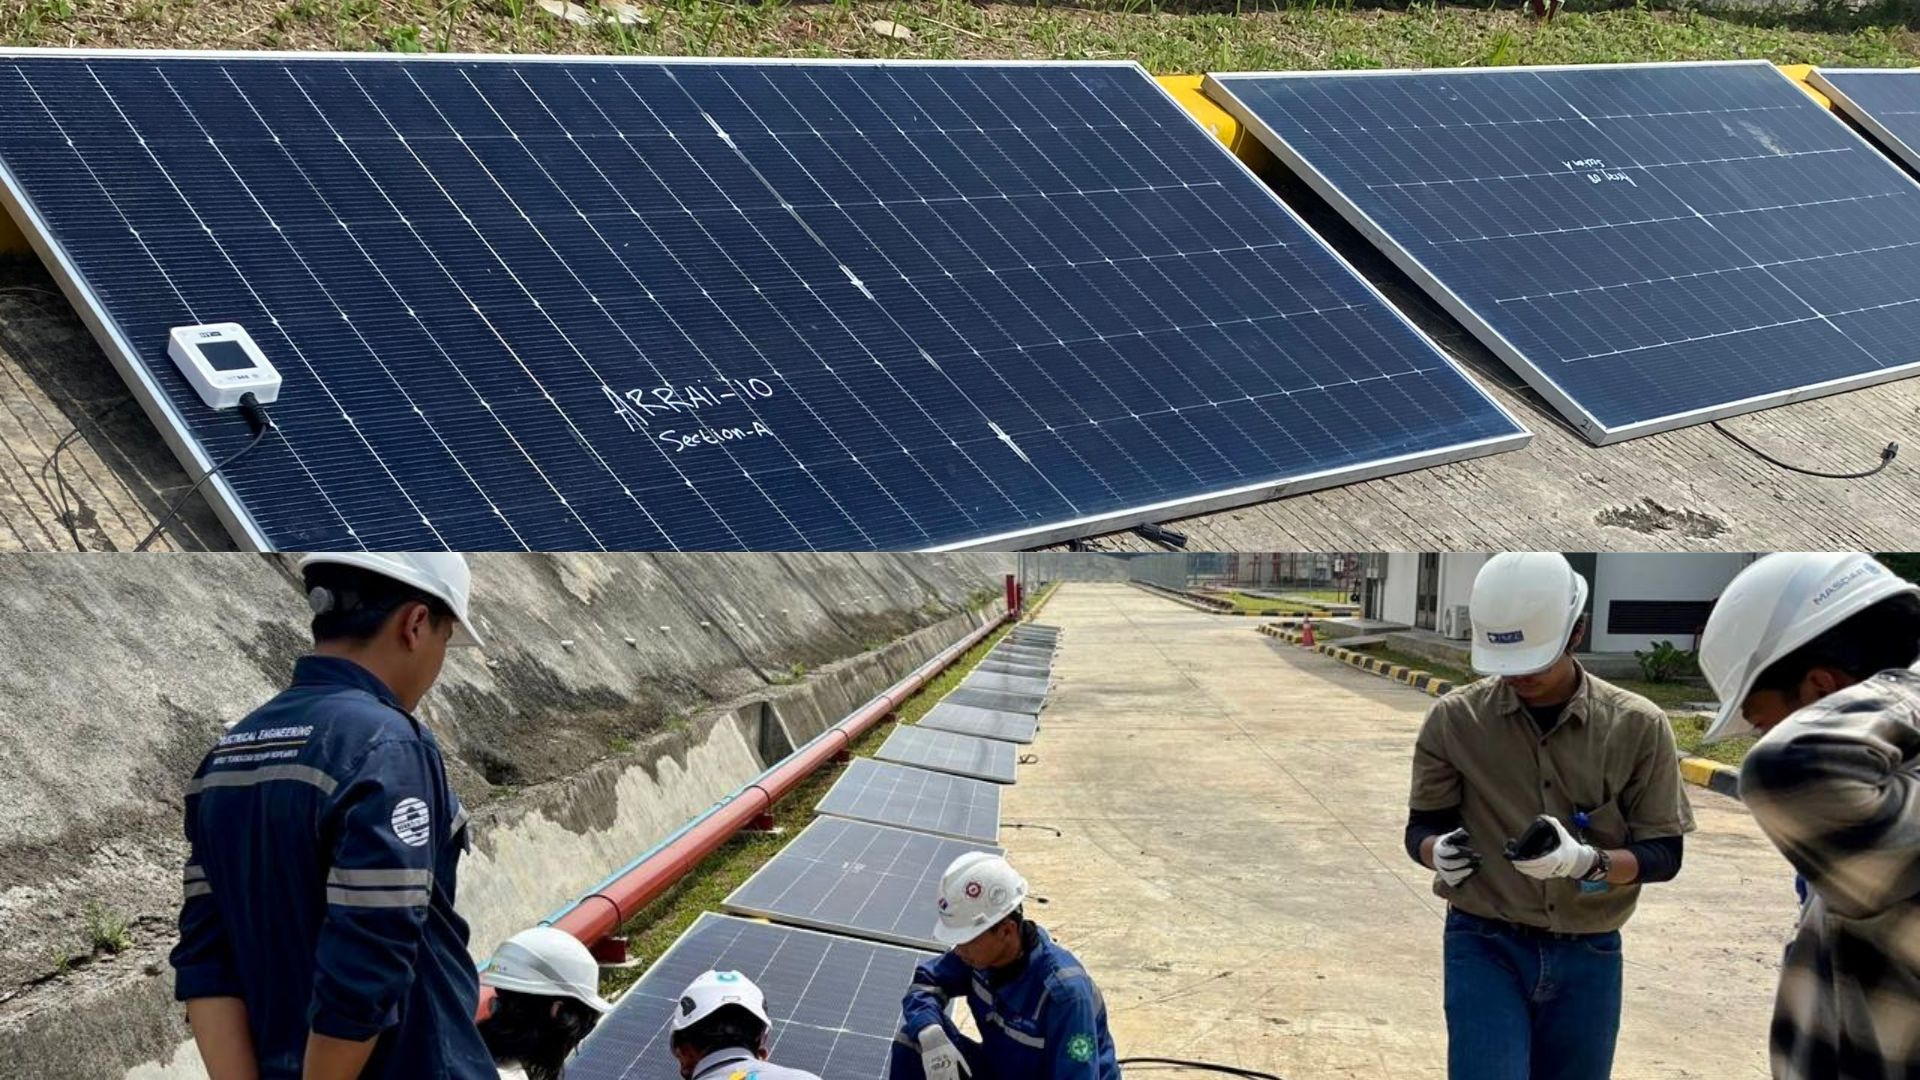
\includegraphics[width=0.80\linewidth]{JKM560N-72HL4-BDV}
\caption{Modul PV JKM560N-72HL4-BDV.}
\label{gbr:modul_produk}
\end{figure}

\begin{table}[H]
\caption{Parameter \textit{datasheet} modul JKM560N pada STC}
\label{tab:datasheet}
\centering
\begin{tabular}{lc}
\toprule
\textbf{Parameter} & \textbf{Nilai} \\
\midrule
Daya maksimum ($P_{max}$)                  & 560 Wp \\
Tegangan \textit{open-circuit} ($V_{oc}$)  & 50,67 V \\
Arus \textit{short-circuit} ($I_{sc}$)     & 14,13 A \\
Tegangan pada MPP ($V_{mp}$)               & 41,95 V \\
Arus pada MPP ($I_{mp}$)                   & 13,35 A \\
Jumlah sel                                 & 144 (2$\times$72) \\
Toleransi daya                             & 0~+3\% \\
Koefisien temperatur $P_{max}$             & $-0,30\%/^{\circ}$C \\
\bottomrule
\end{tabular}
\end{table}

Modul-modul tersebut diangkat dari PLTS Terapung Cirata dan dibawa ke area
\textit{onshore} di lingkungan \textit{warehouse} untuk dilakukan pengujian
dengan mempertimbangkan kondisi cuaca dan menjaga keseragaman azimut antar
pengujian. Dokumentasi modul yang diuji ditunjukkan pada
Gambar~\ref{gbr:foto_modul}.

\begin{figure}[H]
\centering
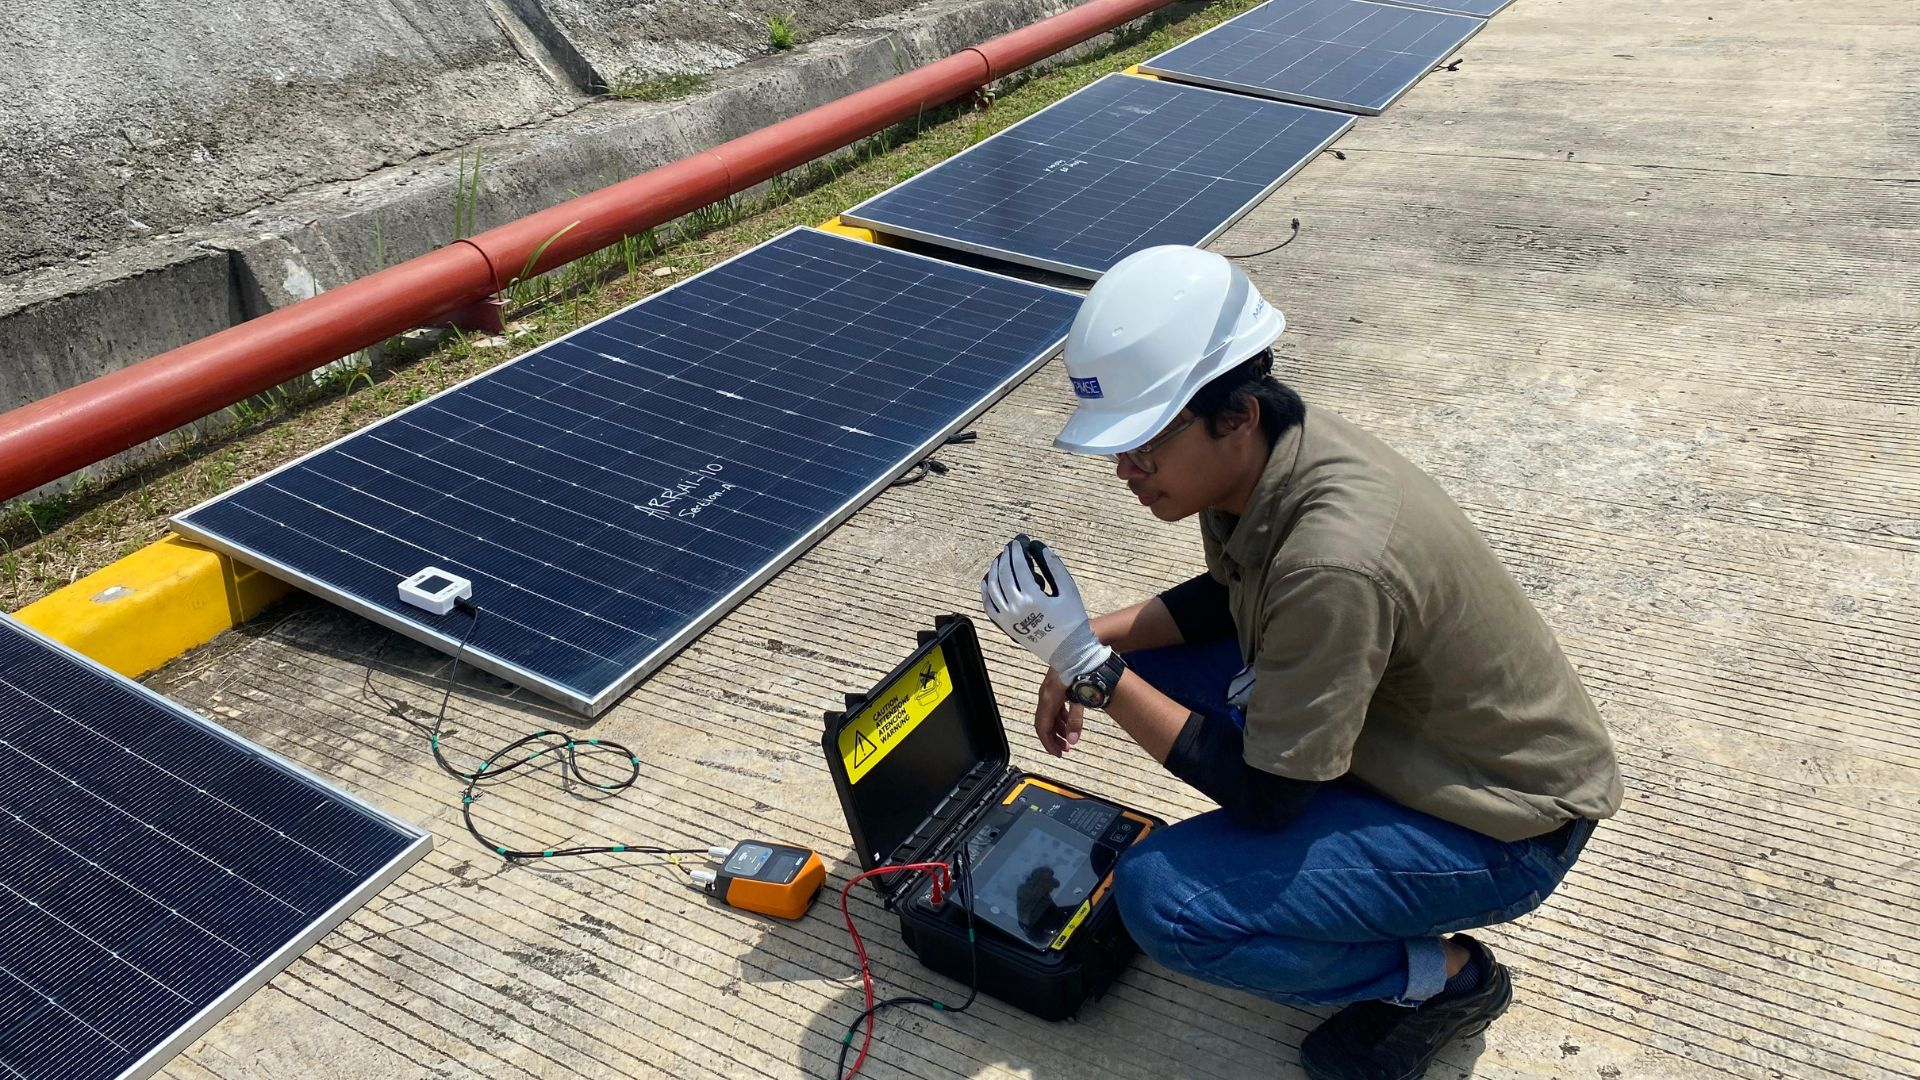
\includegraphics[width=0.80\linewidth]{foto-modul-onshore}
\caption{Modul PV yang diuji secara \textit{onshore}.}
\label{gbr:foto_modul}
\end{figure}

Pengujian kurva I--V dilakukan menggunakan HT Instruments I-V600, yaitu
\textit{I--V curve tracer} yang digunakan untuk pengujian performa modul dan
\textit{string} PV di lapangan. Alat ini mendukung pengujian parameter
$V_{oc}$ dan $I_{sc}$ pada kondisi operasi, serta digunakan bersama pembacaan
irradiansi dan temperatur modul untuk memperoleh parameter yang dikoreksi ke
kondisi STC. Data hasil pengukuran kemudian diolah melalui HTAgora sebagai
perangkat lunak terintegrasi dari I-V600. Skema koneksi pengujian ditunjukkan
pada Gambar~\ref{gbr:setup_uji}.

\begin{figure}[H]
\centering
\begin{tikzpicture}[x=1cm,y=1cm,>=Latex,font=\scriptsize]
\node[draw, rectangle, minimum width=2.2cm, minimum height=1.2cm, line width=0.6pt, fill=blue!8, align=center] (mod) at (0,0) {Modul PV \\ JKM560N};
\node[draw, rectangle, minimum width=2.2cm, minimum height=1.2cm, line width=0.6pt, fill=gray!10, align=center] (tracer) at (3.3,0) {I--V Curve Tracer};
\node[draw, rectangle, minimum width=1.8cm, minimum height=1.2cm, line width=0.6pt, fill=gray!10, align=center] (lap) at (6.3,0) {Laptop \\ Perangkat Lunak};
\node[draw, rectangle, minimum width=1.4cm, minimum height=0.6cm, line width=0.6pt, align=center] (sens) at (3.3,-1.6) {Sensor \\ $G, T$};

\draw[line width=0.7pt] ([yshift=2.5mm]mod.east) -- ([yshift=2.5mm]tracer.west) node[midway, above=-1pt, font=\scriptsize] {$+$};
\draw[line width=0.7pt] ([yshift=-2.5mm]mod.east) -- ([yshift=-2.5mm]tracer.west) node[midway, below=-1pt, font=\scriptsize] {$-$};
\draw[line width=0.7pt] (tracer.east) -- (lap.west) node[midway, above=-1pt, font=\scriptsize] {USB};
\draw[line width=0.7pt] (sens.north) -- (tracer.south);
\end{tikzpicture}
\caption{Skema koneksi alat pengujian kurva I--V.}
\label{gbr:setup_uji}
\end{figure}

Setiap modul terhubung ke \textit{tracer} melalui terminal positif dan negatif.
Sensor irradiansi dan temperatur dipasang di sebelah modul untuk membaca
kondisi pengujian secara \textit{real-time}. Pengukuran dilakukan dengan
menjalankan \textit{sweep} tegangan dari kondisi \textit{short-circuit} hingga
\textit{open-circuit} sehingga diperoleh kurva I--V lengkap. Hasil pengukuran
kemudian dikoreksi ke STC mengacu pada prosedur IEC~60891 \cite{iec60891} dan
IEC~61829 \cite{iec61829}. Dokumentasi alat ditunjukkan pada
Gambar~\ref{gbr:foto_tracer}.

\begin{figure}[H]
\centering
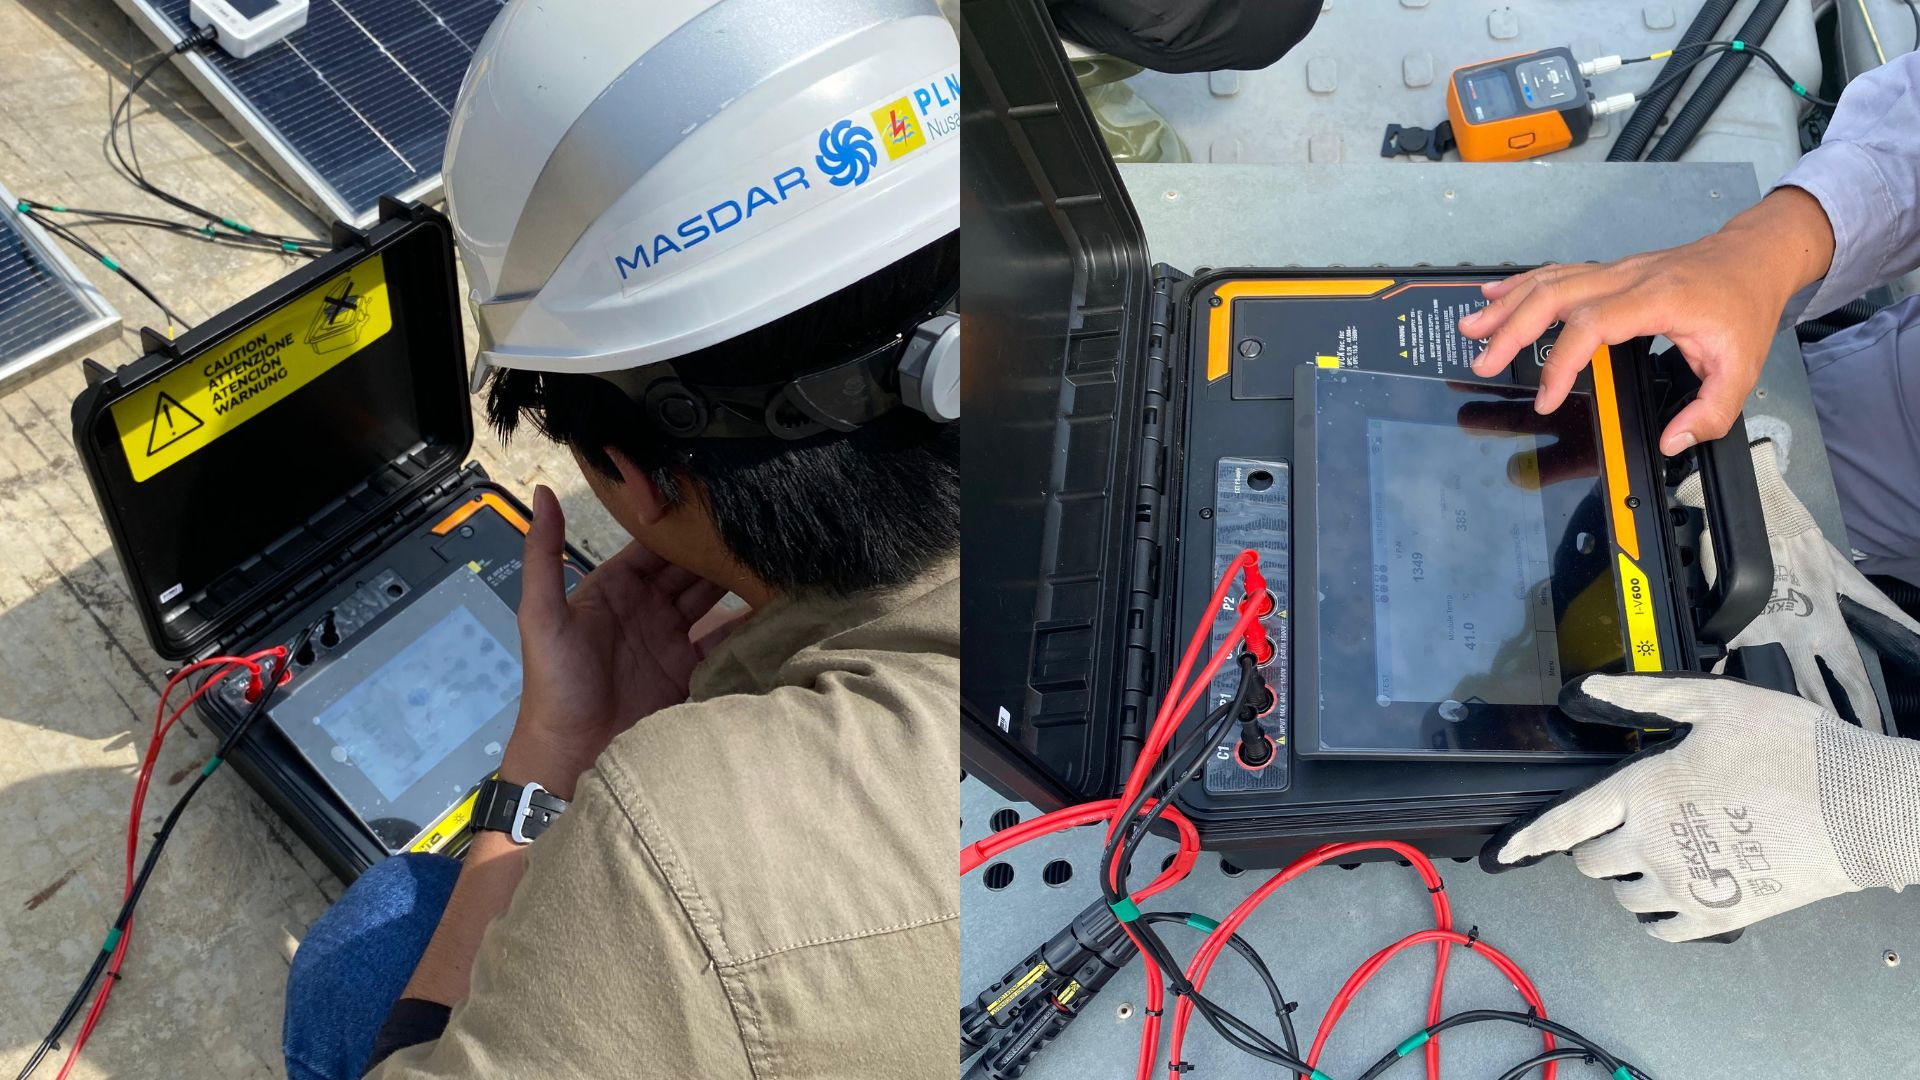
\includegraphics[width=0.80\linewidth]{foto-iv-curve-tracer}
\caption{Alat pengujian \textit{I--V curve tracer}.}
\label{gbr:foto_tracer}
\end{figure}

\section{Tahapan Pengolahan Data}

Pengolahan data dilakukan dalam empat tahap. Alur tahapan ditunjukkan pada
Gambar~\ref{gbr:alur_analisis}.

\begin{figure}[H]
\centering
\begin{tikzpicture}[x=1cm,y=1cm,>=Latex,font=\scriptsize, node distance=0.5cm]
\node[draw, rectangle, rounded corners=2pt, minimum width=7.0cm, minimum height=0.7cm, fill=blue!8, line width=0.5pt] (t1) at (0,3) {Tahap 1: Deviasi parameter terhadap \textit{nameplate}};
\node[draw, rectangle, rounded corners=2pt, minimum width=7.0cm, minimum height=0.7cm, fill=blue!8, line width=0.5pt] (t2) at (0,2) {Tahap 2: Analisis Fill Factor};
\node[draw, rectangle, rounded corners=2pt, minimum width=7.0cm, minimum height=0.7cm, fill=blue!8, line width=0.5pt] (t3) at (0,1) {Tahap 3: Analisis indikator $R_{VM}$ dan $R_{IM}$};
\node[draw, rectangle, rounded corners=2pt, minimum width=7.0cm, minimum height=0.7cm, fill=blue!8, line width=0.5pt] (t4) at (0,0) {Tahap 4: Interpretasi pola degradasi dan implikasi O\&M};
\draw[arr] (t1) -- (t2);
\draw[arr] (t2) -- (t3);
\draw[arr] (t3) -- (t4);
\end{tikzpicture}
\caption{Alur tahapan pengolahan data pengujian.}
\label{gbr:alur_analisis}
\end{figure}

Tahap pertama melakukan perbandingan parameter terukur terhadap nilai
\textit{nameplate}. Deviasi dihitung menggunakan
persamaan~\eqref{eq:deviasi}.
\begin{equation}
\Delta P_{max}\,(\%) =
\frac{P_{max,\text{ukur}} - P_{max,\text{nameplate}}}{P_{max,\text{nameplate}}}
\times 100\%
\label{eq:deviasi}
\end{equation}

Perhitungan yang sama dilakukan untuk parameter $V_{oc}$, $I_{sc}$, $V_{mp}$,
dan $I_{mp}$. Kriteria evaluasi awal mengacu pada toleransi pabrikan 0~+3\% dan
batas penurunan daya 5\% yang digunakan sebagai \textit{screening criterion}
performa daya dari kerangka IEC~61215. Keputusan pemasangan kembali tetap
memerlukan pemeriksaan keselamatan tambahan.

Tahap kedua menghitung Fill Factor menggunakan persamaan~\eqref{eq:ff} dan
membandingkannya dengan $FF$ referensi dari parameter \textit{datasheet}.
Penurunan $FF$ digunakan sebagai indikator perubahan resistansi internal modul.

Tahap ketiga menghitung indikator $R_{VM}$ dan $R_{IM}$ menggunakan
persamaan~\eqref{eq:rvm} dan \eqref{eq:rim}. Distribusi kedua indikator
dianalisis untuk mengidentifikasi pola degradasi yang dominan. Perbedaan
rata-rata antara kelompok Ok dan Not Ok dievaluasi menggunakan
Welch \textit{t-test}. Hasil uji statistik digunakan sebagai analisis pendukung
karena jumlah data antarkelompok tidak seimbang dan kondisi irradiansi saat
pengujian tidak seragam.

Tahap keempat melakukan interpretasi pola degradasi dan mengaitkannya dengan
implikasi pada level sistem dengan mempertimbangkan karakteristik
\textit{open-circuit fault} dan \textit{bypassed-module fault} yang dirangkum
pada Tabel~\ref{tab:fault_signature}. Hasil pengujian I--V memberikan dasar
elektrik awal, tetapi keputusan O\&M tetap perlu mempertimbangkan
\textit{insulation resistance test}, inspeksi visual, dan prosedur perusahaan.
% !TEX root = ../main.tex
% =========================================================
% bab4.tex - HASIL DAN PEMBAHASAN
% Memerlukan tambahan paket: booktabs, pgfplots
% (lihat preambles_tambahan.tex).
% =========================================================

\chapter[HASIL DAN PEMBAHASAN]{\\ HASIL DAN PEMBAHASAN}

Bab ini memuat hasil pengolahan data pengujian kurva I--V modul PV
pasca-terendam beserta pembahasannya. Pembahasan disusun mulai dari
karakteristik data pengujian, kondisi pengukuran dan catatan irradiansi,
analisis status kelayakan berdasarkan $P_{max}$ STC, analisis deviasi parameter
terhadap \textit{nameplate}, analisis Fill Factor, analisis indikator $R_{VM}$
dan $R_{IM}$, interpretasi pola degradasi, serta implikasinya terhadap kegiatan
\textit{operation and maintenance}.

% ---------------------------------------------------------
\section{Karakteristik Data Pengujian}
% ---------------------------------------------------------

Data yang dianalisis terdiri dari 59 data pengujian kurva I--V. Data lengkap
hasil pengujian kurva I--V disajikan pada Lampiran~1, sedangkan bab ini hanya
memuat ringkasan parameter utama yang digunakan dalam analisis. Berdasarkan
keluaran perangkat lunak pengolah data, 6 data pengujian (10,17\%) memperoleh
status Ok, sedangkan 53 data pengujian (89,83\%) memperoleh status Not Ok.
Ringkasan status tersebut ditunjukkan pada Tabel~\ref{tab:status_pengujian}.
Status Ok/Not Ok merupakan hasil \textit{screening} performa daya oleh
perangkat lunak dan belum merepresentasikan keputusan akhir kelayakan
operasional.

\begin{table}[H]
\caption{Ringkasan status awal hasil pengujian modul PV}
\label{tab:status_pengujian}
\centering
\begin{tabular}{lcc}
\toprule
\textbf{Status} & \textbf{Jumlah Data} & \textbf{Persentase} \\
\midrule
Ok      & 6  & 10,17\%  \\
Not Ok  & 53 & 89,83\%  \\
\midrule
Total   & 59 & 100,00\% \\
\bottomrule
\end{tabular}
\end{table}

Distribusi $P_{max}$ STC dari seluruh data pengujian ditunjukkan pada
Gambar~\ref{gbr:dist_pmax}. Kelompok Ok terkonsentrasi pada kisaran 563--573~W,
sedangkan kelompok Not Ok berada pada kisaran 479--537~W. Rata-rata $P_{max}$
STC seluruh data adalah 508,47~W, sedangkan rata-rata kelompok Not Ok adalah
501,6~W.

\begin{figure}[H]
\centering
\begin{tikzpicture}
\begin{axis}[
    width=0.85\linewidth,
    height=0.30\textheight,
    xmin=460, xmax=590,
    ymin=0, ymax=21,
    xlabel={$P_{max}$ STC (W)},
    ylabel={Jumlah Data},
    grid=both,
    minor tick num=1,
    ybar,
    bar width=4pt,
    legend style={font=\scriptsize, at={(0.02,0.98)}, anchor=north west}
]
\addplot[fill=red!50, draw=red!80!black] coordinates {
    (475,1) (485,7) (495,15) (505,19) (515,6) (525,3) (535,2)
};
\addlegendentry{Not Ok}
\addplot[fill=blue!50, draw=blue!80!black] coordinates {
    (565,2) (575,4)
};
\addlegendentry{Ok}
\addplot[gray, dashed, no marks, line width=0.8pt] coordinates {(560,0) (560,21)};
\node[font=\scriptsize] at (axis cs:560,20.0) {Nominal 560 W};
\end{axis}
\end{tikzpicture}
\caption{Distribusi $P_{max}$ STC pada 59 data pengujian.}
\label{gbr:dist_pmax}
\end{figure}

% ---------------------------------------------------------
\section{Kondisi Pengukuran dan Catatan Irradiansi}
% ---------------------------------------------------------

Kondisi irradiansi saat pengukuran menjadi aspek penting dalam interpretasi
hasil. Tabel~\ref{tab:kondisi_irradiance} menunjukkan bahwa kelompok Ok diuji
pada irradiansi yang lebih rendah dibandingkan kelompok Not Ok. Perbedaan ini
perlu diperhatikan karena koreksi kurva I--V ke STC dari irradiansi rendah
dapat memiliki ketidakpastian yang lebih besar. Oleh sebab itu, status Ok
sebaiknya dikonfirmasi melalui pengujian ulang pada irradiansi yang lebih
representatif sebelum dijadikan dasar keputusan pemasangan kembali.

\begin{table}[H]
\caption{Ringkasan irradiansi pengujian pada setiap kelompok}
\label{tab:kondisi_irradiance}
\centering
\begin{tabular}{lcccc}
\toprule
\textbf{Kelompok} & \textbf{$n$} & \textbf{Min.} & \textbf{Maks.} &
\textbf{Rata-rata} \\
 & & \multicolumn{3}{c}{\textbf{Irradiansi \textit{Front} (W/m$^2$)}} \\
\midrule
Ok      & 6  & 198 & 265 & 232,8 \\
Not Ok  & 53 & 737 & 980 & 887,2 \\
\midrule
Total   & 59 & 198 & 980 & 820,6 \\
\bottomrule
\end{tabular}
\end{table}

% ---------------------------------------------------------
\section{Analisis Status Kelayakan Berdasarkan \texorpdfstring{$P_{max}$}{Pmax} STC}
% ---------------------------------------------------------

Status Ok dan Not Ok yang dihasilkan oleh perangkat lunak pengolah data
merupakan hasil \textit{screening} performa daya yang membandingkan $P_{max}$
STC terukur terhadap nilai \textit{nameplate} modul JKM560N-72HL4-BDV sebesar
560~W. Kelompok Ok memiliki rata-rata $P_{max}$ STC di atas nilai nominal,
sedangkan kelompok Not Ok memiliki rata-rata $P_{max}$ STC sebesar 501,6~W atau
sekitar 10,4\% di bawah nilai \textit{nameplate}. Penurunan tersebut
menunjukkan bahwa modul pada kelompok Not Ok mengalami penurunan performa daya
yang substansial terhadap spesifikasi pabrikan.

Status Not Ok tidak secara langsung menentukan jenis kerusakan fisik modul.
Keputusan pemasangan kembali tetap memerlukan pemeriksaan lanjutan, terutama
\textit{insulation resistance test} dan inspeksi visual, mengingat modul
memiliki riwayat terendam. Enam data Ok dapat dipertimbangkan sebagai kandidat
modul yang masih memenuhi kriteria performa daya, tetapi statusnya perlu
dikonfirmasi melalui pengujian ulang pada irradiansi yang lebih representatif
karena keenam data tersebut diperoleh pada irradiansi rendah (rata-rata
232,8~W/m$^2$).

% ---------------------------------------------------------
\section{Analisis Deviasi Parameter terhadap Nameplate}
% ---------------------------------------------------------

Deviasi parameter terhadap nilai \textit{nameplate} dihitung menggunakan
persamaan~\eqref{eq:deviasi_indikator}, dengan $X_{\text{ref}}$ adalah nilai
parameter pada \textit{datasheet} modul JKM560N-72HL4-BDV, yaitu
$P_{max,\text{ref}} = 560$~W, $V_{mp,\text{ref}} = 41{,}95$~V,
$I_{mp,\text{ref}} = 13{,}35$~A, $V_{oc,\text{ref}} = 50{,}67$~V, dan
$I_{sc,\text{ref}} = 14{,}13$~A. Deviasi ini menjadi dasar pembacaan arah
perubahan parameter elektrik pada masing-masing kelompok. Nilai positif
menunjukkan bahwa parameter terukur berada di atas nilai \textit{datasheet},
sedangkan nilai negatif menunjukkan penurunan terhadap referensi. Ringkasan
nilai rata-rata parameter dan deviasi terhadap \textit{datasheet} ditampilkan
pada Tabel~\ref{tab:deviasi}.

\begin{table}[H]
\caption{Perbandingan parameter rata-rata terhadap \textit{datasheet}}
\label{tab:deviasi}
\centering
\begin{tabular}{lccc}
\toprule
\textbf{Parameter} & \textbf{Datasheet} & \textbf{Ok} & \textbf{Not Ok} \\
\midrule
$P_{max}$ (W)         & 560   & 568,8      & 501,6      \\
$\Delta P_{max}$ (\%) & 0     & $+$1,6     & $-$10,4    \\
$V_{oc}$ (V)          & 50,67 & 52,03      & 49,59      \\
$\Delta V_{oc}$ (\%)  & 0     & $+$2,7     & $-$2,1     \\
$I_{sc}$ (A)          & 14,13 & 13,33      & 12,92      \\
$\Delta I_{sc}$ (\%)  & 0     & $-$5,6     & $-$8,5     \\
$V_{mp}$ (V)          & 41,95 & 44,92      & 40,40      \\
$\Delta V_{mp}$ (\%)  & 0     & $+$7,1     & $-$3,7     \\
$I_{mp}$ (A)          & 13,35 & 12,67      & 12,41      \\
$\Delta I_{mp}$ (\%)  & 0     & $-$5,1     & $-$7,0     \\
\bottomrule
\end{tabular}
\end{table}

Tabel~\ref{tab:deviasi} menunjukkan bahwa kelompok Ok memiliki $P_{max}$
rata-rata 568,8~W ($\Delta P_{max} = +1{,}6\%$), yang masih berada dalam
toleransi daya positif pabrikan. Sebaliknya, kelompok Not Ok memiliki $P_{max}$
rata-rata 501,6~W ($\Delta P_{max} = -10{,}4\%$). Parameter $V_{oc}$ pada
kelompok Ok berada di atas nilai \textit{datasheet}, sedangkan pada kelompok
Not Ok berada di bawahnya. Perbedaan yang lebih menonjol terlihat pada $V_{mp}$:
kelompok Ok memiliki rata-rata 44,92~V ($\Delta V_{mp} = +7{,}1\%$), sedangkan
kelompok Not Ok hanya 40,40~V ($\Delta V_{mp} = -3{,}7\%$). Penurunan $V_{mp}$
yang lebih besar dibandingkan penurunan $V_{oc}$ pada kelompok Not Ok
mengindikasikan bahwa perubahan performa lebih dominan terjadi pada sisi
tegangan operasi, terutama di sekitar titik daya maksimum. Sementara itu,
$I_{sc}$ dan $I_{mp}$ pada kedua kelompok sama-sama berada di bawah nilai
\textit{datasheet}, sehingga penurunan arus tidak sepenuhnya spesifik hanya
pada kelompok Not Ok. Deviasi ini selanjutnya digunakan sebagai dasar pembacaan
arah perubahan indikator $R_{VM}$ dan $R_{IM}$.

% ---------------------------------------------------------
\section{Analisis Fill Factor}
% ---------------------------------------------------------

Hasil perhitungan Fill Factor untuk seluruh data pengujian ditunjukkan pada
Gambar~\ref{gbr:ff_dist}. Nilai $FF$ referensi dari \textit{datasheet} adalah
0,7871, dihitung dari $P_{max}/(V_{oc}\cdot I_{sc}) = 560/(50{,}67\times14{,}13)$.

\begin{figure}[H]
\centering
\begin{tikzpicture}
\begin{axis}[
    width=0.85\linewidth,
    height=0.30\textheight,
    xmin=0, xmax=60,
    ymin=0.72, ymax=0.85,
    xlabel={Urutan Data Pengujian},
    ylabel={Fill Factor},
    grid=both,
    minor tick num=1,
    legend style={font=\scriptsize, at={(0.98,0.02)}, anchor=south east},
    only marks
]
\addplot[mark=*, mark size=1.5pt, blue!80!black] coordinates {
    (1,0.8100) (2,0.8300) (3,0.8300) (4,0.8200) (5,0.8100) (6,0.8100)
};
\addlegendentry{Ok}
\addplot[mark=triangle*, mark size=1.5pt, red!80!black] coordinates {
    (7,0.7900) (8,0.7900) (9,0.7800) (10,0.7900) (11,0.7800) (12,0.7800)
    (13,0.7800) (14,0.7800) (15,0.7800) (16,0.7800) (17,0.8000) (18,0.7800)
    (19,0.7800) (20,0.7800) (21,0.7700) (22,0.7800) (23,0.7900) (24,0.7900)
    (25,0.8000) (26,0.7800) (27,0.7900) (28,0.7700) (29,0.7800) (30,0.7900)
    (31,0.7800) (32,0.7800) (33,0.7800) (34,0.7800) (35,0.7900) (36,0.7800)
    (37,0.7800) (38,0.7900) (39,0.7900) (40,0.7700) (41,0.7800) (42,0.7700)
    (43,0.7700) (44,0.7900) (45,0.7900) (46,0.7900) (47,0.7700) (48,0.7900)
    (49,0.8000) (50,0.8000) (51,0.8000) (52,0.7900) (53,0.7700) (54,0.7900)
    (55,0.7900) (56,0.7800) (57,0.7900) (58,0.7900) (59,0.7300)
};
\addlegendentry{Not Ok}
\addplot[gray, dashed, no marks, line width=0.8pt, domain=0:60] {0.7871};
\node[font=\scriptsize] at (axis cs:50,0.7920) {$FF$ \textit{datasheet}};
\end{axis}
\end{tikzpicture}
\caption{Distribusi Fill Factor untuk 59 data pengujian.}
\label{gbr:ff_dist}
\end{figure}

Pada Gambar~\ref{gbr:ff_dist} terlihat bahwa kelompok Ok memiliki $FF$
rata-rata 0,818, sedangkan kelompok Not Ok memiliki $FF$ rata-rata 0,783. Nilai
rata-rata kelompok Not Ok berada sedikit di bawah nilai referensi
\textit{datasheet}, meskipun beberapa data Not Ok masih berada di sekitar nilai
referensi. $FF$ lebih tepat digunakan sebagai indikator perubahan bentuk kurva
I--V, bukan sebagai satu-satunya indikator kelayakan modul. Penurunan $FF$ pada
sebagian data Not Ok konsisten dengan kemungkinan peningkatan resistansi seri
($R_s$), degradasi kontak, korosi interkoneksi, atau mekanisme lain yang
menurunkan kualitas titik daya maksimum. Mekanisme fisik tersebut belum dapat
dipastikan hanya dari data I--V sehingga diperlukan pemeriksaan tambahan
seperti inspeksi visual, \textit{insulation resistance test}, termografi, atau
elektroluminesensi.

% ---------------------------------------------------------
\section{Analisis Indikator \texorpdfstring{$R_{VM}$}{RVM} dan \texorpdfstring{$R_{IM}$}{RIM}}
% ---------------------------------------------------------

Indikator $R_{VM}$ dan $R_{IM}$ dihitung untuk setiap data pengujian
menggunakan persamaan~\eqref{eq:rvm} dan \eqref{eq:rim}. Sebaran kedua
indikator pada bidang $R_{VM}$--$R_{IM}$ ditunjukkan pada
Gambar~\ref{gbr:scatter_rvm_rim}.

\begin{figure}[H]
\centering
\begin{tikzpicture}
\begin{axis}[
    width=0.85\linewidth,
    height=0.32\textheight,
    xmin=0.77, xmax=0.88,
    ymin=0.92, ymax=1.00,
    xlabel={$R_{VM} = V_{mp}/V_{oc}$},
    ylabel={$R_{IM} = I_{mp}/I_{sc}$},
    grid=both,
    minor tick num=1,
    legend style={font=\scriptsize, at={(0.02,0.02)}, anchor=south west},
    only marks
]
\addplot[mark=*, mark size=2pt, blue!80!black] coordinates {
    (0.8700,0.9350) (0.8637,0.9653) (0.8541,0.9716)
    (0.8654,0.9465) (0.8615,0.9426) (0.8646,0.9403)
};
\addlegendentry{Ok}
\addplot[mark=triangle*, mark size=1.6pt, red!80!black, opacity=0.7] coordinates {
    (0.8111,0.9699) (0.8124,0.9670) (0.8156,0.9546) (0.8134,0.9672)
    (0.8117,0.9613) (0.8247,0.9477) (0.8049,0.9696) (0.8167,0.9558)
    (0.8126,0.9587) (0.8216,0.9446) (0.8152,0.9828) (0.8160,0.9556)
    (0.8080,0.9686) (0.8303,0.9408) (0.8140,0.9420) (0.8140,0.9566)
    (0.8064,0.9818) (0.8147,0.9652) (0.8257,0.9696) (0.8000,0.9739)
    (0.8164,0.9656) (0.8147,0.9486) (0.8240,0.9513) (0.8350,0.9431)
    (0.8169,0.9552) (0.7980,0.9837) (0.8147,0.9552) (0.8000,0.9755)
    (0.8131,0.9673) (0.7948,0.9789) (0.8199,0.9556) (0.8140,0.9652)
    (0.8140,0.9652) (0.8124,0.9527) (0.8120,0.9636) (0.8163,0.9483)
    (0.8191,0.9462) (0.8206,0.9584) (0.8245,0.9521) (0.8182,0.9632)
    (0.8248,0.9355) (0.8093,0.9763) (0.8150,0.9768) (0.8167,0.9787)
    (0.8333,0.9560) (0.8296,0.9550) (0.8000,0.9635) (0.8316,0.9455)
    (0.8061,0.9773) (0.8145,0.9573) (0.8084,0.9722) (0.8258,0.9536)
    (0.7800,0.9359)
};
\addlegendentry{Not Ok}
\end{axis}
\end{tikzpicture}
\caption{Sebaran indikator $R_{VM}$ dan $R_{IM}$ untuk 59 data pengujian.}
\label{gbr:scatter_rvm_rim}
\end{figure}

Pada Gambar~\ref{gbr:scatter_rvm_rim} terlihat bahwa kelompok Ok terkonsentrasi
pada nilai $R_{VM}$ yang lebih tinggi, sedangkan kelompok Not Ok berada pada
rentang $R_{VM}$ yang lebih rendah. Rata-rata $R_{VM}$ kelompok Ok adalah
0,863, sedangkan kelompok Not Ok adalah 0,815. Sebaliknya, nilai $R_{IM}$ kedua
kelompok saling tumpang tindih, dengan rata-rata 0,950 pada kelompok Ok dan
0,961 pada kelompok Not Ok. Pola ini menunjukkan bahwa pemisahan kelompok
terutama terjadi pada sisi tegangan, konsisten dengan temuan pada
Tabel~\ref{tab:deviasi}.

Nilai referensi $R_{VM}$ dan $R_{IM}$ dihitung dari parameter \textit{datasheet}
modul JKM560N-72HL4-BDV:
\[
R_{VM,\text{ref}} = \frac{V_{mp,\text{ref}}}{V_{oc,\text{ref}}}
  = \frac{41{,}95}{50{,}67} = 0{,}828, \qquad
R_{IM,\text{ref}} = \frac{I_{mp,\text{ref}}}{I_{sc,\text{ref}}}
  = \frac{13{,}35}{14{,}13} = 0{,}945.
\]
Deviasi masing-masing indikator terhadap referensi dihitung menggunakan
persamaan~\eqref{eq:deviasi_indikator} dan dirangkum pada
Tabel~\ref{tab:rvm_rim_dev}.

\begin{table}[H]
\caption{Deviasi indikator $R_{VM}$ dan $R_{IM}$ terhadap nilai referensi
         \textit{datasheet}}
\label{tab:rvm_rim_dev}
\centering
\begin{tabular}{lccccc}
\toprule
\textbf{Indikator} & \textbf{Ref.} &
\textbf{Ok} & \textbf{Not Ok} &
\textbf{$\Delta$Ok (\%)} & \textbf{$\Delta$Not Ok (\%)} \\
\midrule
$R_{VM}$ & 0,828 & 0,863 & 0,815 & $+$4,23 & $-$1,57 \\
$R_{IM}$ & 0,945 & 0,950 & 0,961 & $+$0,55 & $+$1,71 \\
\bottomrule
\end{tabular}
\end{table}

Tabel~\ref{tab:rvm_rim_dev} menunjukkan bahwa $\Delta R_{VM}$ kelompok Not Ok
bernilai $-1{,}57\%$, artinya rasio tegangan operasi terhadap $V_{oc}$ menurun
terhadap nilai referensi. Sebaliknya, $\Delta R_{IM}$ kelompok Not Ok bernilai
$+1{,}71\%$ sehingga tidak menunjukkan penurunan pada sisi arus. Berdasarkan
persamaan~\eqref{eq:delta_v} dan \eqref{eq:delta_i}, diperoleh
$\delta_V = \max(0,\,1{,}57\%) = 1{,}57\%$ dan
$\delta_I = \max(0,\,-1{,}71\%) = 0{,}00\%$ untuk kelompok Not Ok. Indeks
dominasi dihitung menggunakan persamaan~\eqref{eq:dominasi_tegangan} dan
\eqref{eq:dominasi_arus}, dan hasilnya dirangkum pada
Tabel~\ref{tab:dominasi_penurunan}.

\begin{table}[H]
\caption{Indeks dominasi penurunan indikator sisi tegangan dan arus pada
         kelompok Not Ok}
\label{tab:dominasi_penurunan}
\centering
\begin{tabular}{lcccc}
\toprule
\textbf{Kelompok} & \textbf{$\delta_V$ (\%)} & \textbf{$\delta_I$ (\%)} &
\textbf{$D_V$} & \textbf{$D_I$} \\
\midrule
Not Ok & 1,57 & 0,00 & 1,00 & 0,00 \\
\bottomrule
\end{tabular}
\end{table}

Nilai $D_V = 1{,}00$ yang diperoleh pada Tabel~\ref{tab:dominasi_penurunan}
menunjukkan bahwa penurunan indikator yang terdeteksi lebih dominan terjadi
pada sisi tegangan. Hasil ini konsisten dengan $\delta_I = 0$ yang muncul
karena $\Delta R_{IM}$ kelompok Not Ok tidak bernilai negatif. Nilai $D_V$ yang
lebih besar menunjukkan bahwa penurunan indikator lebih dominan terjadi pada
sisi tegangan. Hasil ini tidak digunakan untuk menetapkan jenis gangguan secara
final, tetapi untuk membaca arah perubahan parameter elektrik pada kelompok Not
Ok.

Welch \textit{t-test} digunakan untuk membandingkan rata-rata parameter antara
kelompok Ok ($n=6$) dan kelompok Not Ok ($n=53$). Uji ini dipilih karena jumlah
data tidak seimbang dan variansi kedua kelompok tidak diasumsikan sama. Taraf
signifikansi yang digunakan adalah $\alpha=0{,}05$. Hasil uji berfungsi sebagai
pendukung interpretasi indikator, bukan sebagai dasar tunggal kelayakan
operasional.

Untuk setiap parameter $X \in \{P_{max},\,V_{oc},\,I_{sc},\,V_{mp},\,I_{mp},\,
R_{VM},\,R_{IM},\,FF\}$, hipotesis yang diuji adalah:
\begin{equation}
\begin{aligned}
H_0 &: \mu_{\mathrm{Ok},X} = \mu_{\mathrm{NotOk},X},\\
H_1 &: \mu_{\mathrm{Ok},X} \neq \mu_{\mathrm{NotOk},X},
\end{aligned}
\label{eq:hipotesis_welch}
\end{equation}
dengan $\mu_{\mathrm{Ok},X}$ adalah rata-rata parameter $X$ pada kelompok Ok
dan $\mu_{\mathrm{NotOk},X}$ pada kelompok Not Ok. Aturan keputusan dua arah
yang digunakan adalah:
\begin{equation}
p < \alpha \;\Rightarrow\; H_0 \text{ ditolak},\qquad
p \geq \alpha \;\Rightarrow\; H_0 \text{ tidak ditolak}.
\label{eq:keputusan_welch}
\end{equation}

Hasil pengujian ditunjukkan pada Tabel~\ref{tab:ttest}.

\begin{table}[H]
\caption{Hasil Welch \textit{t-test} antara kelompok Ok dan Not Ok}
\label{tab:ttest}
\centering
\begin{tabular}{lcccc}
\toprule
\textbf{Parameter} & \textbf{$t$} & \textbf{$p$-value} &
\textbf{Selisih Ok--Not Ok} & \textbf{Signifikan} \\
\midrule
$P_{max}$ & 26,95   & $<0,001$ & $+$13,4\% & Ya    \\
$V_{oc}$  & 20,13   & $<0,001$ & $+$4,9\%  & Ya    \\
$I_{sc}$  & 3,54    & 0,011    & $+$3,2\%  & Ya    \\
$V_{mp}$  & 27,09   & $<0,001$ & $+$11,2\% & Ya    \\
$I_{mp}$  & 4,15    & 0,001    & $+$2,0\%  & Ya    \\
$R_{VM}$  & 19,00   & $<0,001$ & $+$5,9\%  & Ya    \\
$R_{IM}$  & $-1,66$ & 0,150    & $-$1,1\%  & Tidak \\
$FF$      & 8,17    & $<0,001$ & $+$4,5\%  & Ya    \\
\bottomrule
\end{tabular}
\end{table}

Visualisasi signifikansi ditunjukkan pada Gambar~\ref{gbr:signifikansi_welch}
melalui nilai $-\log_{10}(p)$. Garis putus-putus pada $-\log_{10}(0{,}05)=1{,}301$
merupakan batas keputusan; batang yang melewati garis tersebut menunjukkan
parameter yang signifikan.

\begin{figure}[H]
\centering
\begin{tikzpicture}
\begin{axis}[
    width=0.82\linewidth,
    height=0.34\textheight,
    xbar,
    xmin=0, xmax=3.6,
    bar width=9pt,
    symbolic y coords={%
        $FF$,$R_{IM}$,$R_{VM}$,$I_{mp}$,$V_{mp}$,$I_{sc}$,$V_{oc}$,$P_{max}$},
    ytick=data,
    yticklabel style={font=\small},
    xlabel={$-\log_{10}(p)$},
    xmajorgrids=true,
    minor x tick num=1,
    enlarge y limits=0.12,
    extra x ticks={1.301},
    extra x tick labels={$\alpha{=}0{,}05$},
    extra x tick style={
        grid=major,
        grid style={dashed, gray!70, line width=0.9pt},
        tick label style={font=\scriptsize, gray!70, rotate=90, anchor=west},
        tick style={draw=none},
    },
    legend style={font=\scriptsize, at={(0.98,0.02)}, anchor=south east},
]
%--- Batang signifikan (biru) ---
\addplot[xbar, fill=blue!50, draw=blue!80!black] coordinates {
    (3.000,$P_{max}$)
    (3.000,$V_{oc}$)
    (1.959,$I_{sc}$)
    (3.000,$V_{mp}$)
    (3.000,$I_{mp}$)
    (3.000,$R_{VM}$)
    (3.000,$FF$)
};
\addlegendentry{Signifikan ($p<\alpha$)}
%--- Batang tidak signifikan (merah) ---
\addplot[xbar, fill=red!45, draw=red!80!black] coordinates {
    (0.824,$R_{IM}$)
};
\addlegendentry{Tidak signifikan ($p\geq\alpha$)}
\end{axis}
\end{tikzpicture}
\caption{Signifikansi parameter berdasarkan Welch \textit{t-test}.}
\label{gbr:signifikansi_welch}
\end{figure}

Berdasarkan persamaan~\eqref{eq:keputusan_welch} dan Gambar~\ref{gbr:signifikansi_welch},
hampir seluruh parameter berbeda signifikan antara kelompok Ok dan Not Ok,
kecuali $R_{IM}$ ($p=0{,}150\geq\alpha$, $H_0$ tidak ditolak). Indikator
$R_{VM}$ berbeda signifikan ($p<0{,}001$, $H_0$ ditolak), yang mendukung
interpretasi bahwa pemisahan kelompok lebih kuat terjadi pada sisi tegangan
daripada sisi arus. Hasil ini memperkuat temuan pada Tabel~\ref{tab:rvm_rim_dev}
dan konsisten dengan nilai $D_V=1{,}00$ pada Tabel~\ref{tab:dominasi_penurunan}.

% ---------------------------------------------------------
\section{Interpretasi Pola Degradasi}
% ---------------------------------------------------------

Berdasarkan hasil analisis deviasi, indikator $R_{VM}$/$R_{IM}$, indeks
dominasi, dan uji statistik, pola yang paling menonjol pada kelompok Not Ok
adalah penurunan sisi tegangan operasi. Penurunan $P_{max}$ rata-rata sebesar
10,4\% terhadap \textit{nameplate} diikuti oleh $\Delta R_{VM} = -1{,}57\%$
dan $D_V = 1{,}00$, yang menunjukkan bahwa arah penurunan indikator dominan
pada sisi tegangan. Indikator $R_{VM}$ berbeda signifikan antara kelompok Ok
dan Not Ok berdasarkan Welch \textit{t-test}, sedangkan $R_{IM}$ tidak berbeda
signifikan sehingga sisi arus bukan pemisah utama pada dataset ini. Interpretasi
ini dibatasi sebagai indikasi awal berbasis I--V dan tidak digunakan untuk
menetapkan jenis gangguan secara final.

Pola ini konsisten dengan kemungkinan peningkatan resistansi seri, degradasi
kontak, korosi interkoneksi, atau ketidakteraturan karakteristik sel yang
menyebabkan titik daya maksimum bergeser ke tegangan yang lebih rendah. Dalam
model satu dioda, peningkatan $R_s$ dapat menurunkan kualitas daerah
\textit{knee} kurva I--V dan berdampak pada penurunan $FF$
\cite{villalva2009}. Penurunan $I_{sc}$ pada kedua kelompok menunjukkan adanya
komponen penurunan pada sisi arus; akan tetapi, karena $R_{IM}$ tidak
menunjukkan perbedaan signifikan dan $\delta_I = 0$, penurunan arus tidak
menjadi indikator pemisah utama pada dataset ini.

Penyebab fisik degradasi belum dapat dipastikan hanya dari hasil pengujian I--V.
Riwayat perendaman membuat mekanisme berbasis kelembapan menjadi relevan untuk
dipertimbangkan, tetapi pembuktiannya tetap memerlukan data tambahan. Oleh
karena itu, hasil I--V pada analisis ini diposisikan sebagai dasar awal untuk
menentukan prioritas pemeriksaan lanjutan, bukan sebagai bukti tunggal
mengenai jenis kerusakan fisik modul.

% ---------------------------------------------------------
\section{Implikasi terhadap Operation and Maintenance}
% ---------------------------------------------------------

Pola degradasi yang teridentifikasi pada kelompok Not Ok memiliki implikasi
terhadap operasi sistem jika modul tersebut dipasang kembali pada
\textit{string}. Penurunan $V_{mp}$ pada modul Not Ok dapat memengaruhi
tegangan operasi \textit{string} jika modul tersebut tersusun seri dengan modul
lain yang masih normal. Tegangan operasi \textit{string} yang mengandung $N_d$
modul terdegradasi dapat dinyatakan seperti pada
persamaan~\eqref{eq:vstring_deg}.
\begin{equation}
V_{string,\text{deg}} =
\sum_{j=1}^{N_s-N_d} V_{mp,\text{normal}} +
\sum_{j=1}^{N_d} V_{mp,\text{deg}}
\label{eq:vstring_deg}
\end{equation}

Karena $V_{mp,\text{deg}} < V_{mp,\text{normal}}$, peningkatan jumlah modul
terdegradasi menurunkan tegangan operasi \textit{string}. Hasil I--V tidak
cukup untuk dijadikan dasar tunggal keputusan pemasangan kembali modul
pasca-terendam.

Modul-modul yang memperoleh status Not Ok perlu diprioritaskan untuk
pemeriksaan lanjutan sebelum keputusan pemasangan kembali diambil. Pengujian
tahanan isolasi (\textit{insulation resistance test}) menjadi prioritas karena
risiko utama pada modul pasca-terendam bukan hanya penurunan daya, tetapi juga
keselamatan listrik; paparan air dan kelembapan dapat menurunkan tahanan
isolasi dan meningkatkan risiko arus bocor atau \textit{ground fault}
\cite{ketjoy2022,smaGroundFault}. Untuk 6 data pengujian berstatus Ok, status
tersebut perlu dikonfirmasi melalui pengujian ulang pada irradiansi yang lebih
representatif, dan keputusan pemasangan kembali tetap memerlukan hasil
\textit{insulation resistance test} mengingat riwayat perendaman modul. Dengan
demikian, hasil I--V berfungsi sebagai dasar awal untuk memilah modul
berdasarkan performa daya, sedangkan keputusan operasional akhir harus
mempertimbangkan aspek keselamatan isolasi serta prosedur O\&M PLTS Terapung
Cirata.
% !TEX root = ../main.tex
% =========================================================
% bab5.tex - PENUTUP
% =========================================================

\chapter[PENUTUP]{\\ PENUTUP}

\section{Kesimpulan}

Berdasarkan analisis dan pembahasan data hasil pengujian kurva I--V modul PV
pasca-terendam pada PLTS Terapung Cirata, diperoleh beberapa kesimpulan, yaitu:

\begin{enumerate}
    \item Analisis dilakukan terhadap 59 data pengujian kurva I--V modul PV
          pasca-terendam tipe JKM560N-72HL4-BDV yang diuji secara
          \textit{onshore} dengan koreksi parameter ke STC. Karena terdapat
          satu nomor uji yang muncul dua kali, hasil dinyatakan berdasarkan
          data pengujian dan bukan sebagai klaim jumlah modul unik.

    \item Hasil \textit{screening} performa daya oleh perangkat lunak pengolah
          data menunjukkan 6 data (10,17\%) berstatus Ok dan 53 data (89,83\%)
          berstatus Not Ok. Status ini merupakan hasil perbandingan $P_{max}$
          STC terukur terhadap nilai \textit{nameplate} modul dan belum
          merepresentasikan keputusan akhir kelayakan operasional.

    \item Kelompok Not Ok mengalami penurunan rata-rata $P_{max}$ STC menjadi
          sekitar 501,6~W atau sekitar 10,4\% di bawah nilai \textit{nameplate}
          560~W. Penurunan ini menunjukkan bahwa modul pada kelompok Not Ok
          mengalami penurunan performa daya yang substansial terhadap
          spesifikasi pabrikan.

    \item Analisis deviasi indikator $R_{VM}$ dan $R_{IM}$ terhadap nilai
          referensi \textit{datasheet} menghasilkan $\Delta R_{VM} = -1{,}57\%$
          dan $\Delta R_{IM} = +1{,}71\%$ untuk kelompok Not Ok, sehingga
          diperoleh $\delta_V = 1{,}57\%$, $\delta_I = 0{,}00\%$, dan
          $D_V = 1{,}00$. Indikator $R_{VM}$ berbeda signifikan antara kedua
          kelompok berdasarkan Welch \textit{t-test} ($p < 0{,}001$), sedangkan
          $R_{IM}$ tidak berbeda signifikan ($p = 0{,}150$), sehingga pemisahan
          kelompok lebih dominan terjadi pada sisi tegangan.

    \item Pola penurunan sisi tegangan pada kelompok Not Ok konsisten dengan
          kemungkinan peningkatan resistansi seri atau mekanisme degradasi lain
          yang menurunkan tegangan operasi modul. Interpretasi ini dibatasi
          sebagai indikasi awal berbasis I--V dan tidak digunakan untuk
          menetapkan jenis kerusakan fisik modul secara final.

    \item Hasil pengujian I--V tidak cukup menjadi dasar tunggal keputusan
          pemasangan kembali karena aspek keselamatan listrik tidak dapat
          disimpulkan hanya dari parameter kurva I--V, sehingga diperlukan
          pengujian tahanan isolasi dan pemeriksaan keselamatan lanjutan.
\end{enumerate}

\section{Saran}

Berdasarkan hasil analisis yang telah dilakukan, berikut ini adalah saran-saran
yang dapat digunakan sebagai panduan untuk kegiatan dan pengembangan
selanjutnya:

\begin{enumerate}
    \item Melakukan pengujian tahanan isolasi (\textit{insulation resistance
          test}) pada seluruh modul pasca-terendam sebelum keputusan pemasangan
          kembali, karena risiko utama bukan hanya penurunan daya tetapi juga
          keselamatan listrik.

    \item Melengkapi evaluasi dengan inspeksi visual, termografi, dan/atau
          elektroluminesensi jika tersedia untuk mengonfirmasi mekanisme
          degradasi yang teridentifikasi dari parameter elektrik.

    \item Melakukan pengujian ulang pada kondisi irradiansi yang lebih
          representatif untuk data yang diperoleh pada irradiansi rendah,
          khususnya kelompok Ok, sebelum data tersebut dijadikan dasar
          keputusan.

    \item Mendokumentasikan kondisi modul dan riwayat lokasi modul secara
          sistematis agar interpretasi pola degradasi dapat dikaitkan dengan
          kondisi operasi aktual.

    \item Mengintegrasikan hasil pengujian I--V dengan prosedur
          \textit{operation and maintenance} PLTS Terapung Cirata, termasuk
          pemantauan parameter tegangan ($V_{mp}$ dan tegangan
          \textit{string}) sebagai indikator awal adanya modul terdegradasi.
\end{enumerate}

% =========================================================
% daftarpustaka.tex - DAFTAR PUSTAKA
% =========================================================

\clearpage
\phantomsection
\addcontentsline{toc}{chapter}{DAFTAR PUSTAKA}
\renewcommand\bibname{DAFTAR PUSTAKA}

\begin{thebibliography}{99}

\bibitem{worldbankFPV2019}
World Bank Group, ESMAP, and SERIS, \textit{Where Sun Meets Water: Floating Solar Handbook for Practitioners}. Washington, DC, USA: World Bank, 2019. [Online]. Available: \url{https://openknowledge.worldbank.org/entities/publication/645af5c2-9fbc-5575-8fd5-6dbed04e09b4}

\bibitem{ieaFPV2025}
IEA PVPS Task 13, \textit{Floating Photovoltaic Power Plants: A Review of Energy Yield, System Reliability and Operations and Maintenance}. International Energy Agency Photovoltaic Power Systems Programme, 2025. [Online]. Available: \url{https://iea-pvps.org/key-topics/t13-floating-pv-plants-review-2025/}

\bibitem{ketjoy2022}
N. Ketjoy, P. Mensin, and W. Chamsa-ard, ``Impacts on Insulation Resistance of Thin Film Modules: A Case Study of a Flooding of a Photovoltaic Power Plant in Thailand,'' \textit{PLOS ONE}, vol. 17, no. 9, p. e0274839, 2022.

\bibitem{linwu2025}
J.-H. Lin and Y.-K. Wu, ``Simulation and Fault Diagnosis Using Current-Voltage Characteristics of Photovoltaic Systems---A Case Study,'' in \textit{Engineering Proceedings}, vol. 92, no. 1. MDPI, 2025, p. 79.

\bibitem{pei2019}
T. Pei and X. Hao, ``A Fault Detection Method for Photovoltaic Systems Based on Voltage and Current Observation and Evaluation,'' \textit{Energies}, vol. 12, no. 9, p. 1712, 2019.

\bibitem{sugirianta2022}
I. B. K. Sugirianta, I. G. N. A. D. Saputra, I. M. Purbhawa, I. G. K. S. Budarsa, and I. K. Ta, ``Short and Open Circuit Fault Detection in On-Grid Photovoltaic Systems 1MWp Bangli Based on Current and Voltage Observation,'' \textit{Journal of Computer Science and Technology Studies}, vol. 4, no. 2, pp. 105--117, 2022.

\bibitem{nunes2022}
H. G. G. Nunes et al., ``Bypass Diode Effect and Photovoltaic Parameter Estimation under Partial Shading Using a Hill Climbing Neural Network Algorithm,'' \textit{Frontiers in Energy Research}, vol. 10, p. 837540, 2022.

\bibitem{pveducationBypass}
PV Education, ``Bypass Diodes,'' Online, 2024. [Online]. Available: \url{https://www.pveducation.org/pvcdrom/modules-and-arrays/bypass-diodes}

\bibitem{smaGroundFault}
SMA Solar Technology AG, ``Checking the PV System for Ground Faults,'' Online manual, 2024. [Online]. Available: \url{https://manuals.sma.de/SBxx-1VL-40/en-US/391466379.html}

\bibitem{villalva2009}
M. G. Villalva, J. R. Gazoli, and E. R. Filho, ``Comprehensive Approach to Modeling and Simulation of Photovoltaic Arrays,'' \textit{IEEE Transactions on Power Electronics}, vol. 24, no. 5, pp. 1198--1208, 2009.

\bibitem{jinko2022}
JinkoSolar, \textit{Tiger Neo N-type 72HL4-BDV 560--580 Watt Bifacial Module with Dual Glass}. JinkoSolar Co., Ltd., 2022.

\bibitem{iec61215}
IEC, \textit{IEC 61215-1: Terrestrial Photovoltaic (PV) Modules---Design Qualification and Type Approval---Part 1: Test Requirements}. International Electrotechnical Commission, 2021.

\bibitem{iec60891}
IEC, \textit{IEC 60891: Photovoltaic Devices---Procedures for Temperature and Irradiance Corrections to Measured I--V Characteristics}. International Electrotechnical Commission, 2021.

\bibitem{iec61829}
IEC, \textit{IEC 61829: Photovoltaic (PV) Array---On-site Measurement of Current-voltage Characteristics}. International Electrotechnical Commission, 2015.

\bibitem{htiv6002025}
HT Instruments, \textit{I-V600 Professional I-V Curve Tracer up to 1500V,
40ADC}, Rel. 2.01, 2025.

\bibitem{pmse2021}
PT Pembangkitan Jawa Bali Masdar Solar Energi (PT PMSE), \textit{Profil Perusahaan dan Proyek PLTS Terapung Cirata 145 MWac}. Jakarta, Indonesia: PT PMSE, 2021. [Online]. Available: \url{https://pmse.solar/}

\end{thebibliography}
\input{chapters/lampiran1}

\end{document}
